\documentclass[12pt,a4paper,twoside]{book}
\usepackage[utf8]{inputenc}
\usepackage{amsmath}
\usepackage{amsfonts}
\usepackage{amssymb}
\usepackage{graphicx}
\usepackage[inner=3.00cm, outer=2.50cm, top=3.00cm, bottom=3.00cm]{geometry}
\usepackage[slovene]{babel}
\usepackage{babelbib}
\usepackage{titlesec}
\usepackage{listings}
\usepackage{fancyhdr}
\usepackage{eurosym}
\usepackage{url}
\author{Luka Horvat}
\title{Dobre prakse pri razvoju računalniških iger}

\graphicspath{{images/}}
%Paragraph indenting, title spacing and line spacing
\setlength{\parindent}{0pt}
\setlength{\parskip}{1em}
\renewcommand{\baselinestretch}{1.5}

% Remove big chapter text
\titleformat{\chapter}{\bfseries\LARGE}{\thechapter}{1em}{\LARGE\textbf}

% Code listings
\lstdefinestyle{mystyle}{
	numbers=left,
	breaklines=true,
	basicstyle=\footnotesize,
	frame=tb,
	captionpos=b
}
\lstset{style=mystyle}
\renewcommand{\lstlistingname}{Izsek kode}
\renewcommand{\lstlistlistingname}{Seznam izsekov kode}
%\renewcommand{\thelstlisting}{\thesection.\arabic{lstlisting}}

%Header/footer
\pagestyle{fancy}
\fancyhf{}
\fancyfoot[LE, RO]{\thepage}
\renewcommand{\headrulewidth}{0pt}
\renewcommand{\footrulewidth}{0pt}

\fancypagestyle{plain}{%
	\fancyhf{}
	\renewcommand{\headrulewidth}{0pt}
	\fancyfoot[LE, RO]{\thepage}
}

%Initial pages are in Roman numbering
\pagenumbering{Roman}
\begin{document}
	
%First page
\thispagestyle{empty} 
\begin{center}
	{\large 
		UNIVERZA V MARIBORU\\
		FAKULTETA ZA ELEKTROTEHNIKO,\\
		RAČUNALNIŠTVO IN INFORMATIKO\\
	}
	
	\vspace{\fill}
	{\LARGE Luka Horvat}\\
	
	\vspace{1cm}
	\textsc{\textbf{\LARGE DOBRE PRAKSE PRI RAZVOJU RAČUNALNIŠKIH IGER\\}}
	
	\vspace{1cm}
	{\LARGE Magistrsko delo}
	
	\vfill
	{\Large Maribor, februar 2018}
	\newpage
\end{center}

%Empty page
\ \thispagestyle{empty}
\newpage

%Second page
\thispagestyle{empty} 
\begin{center}	
	\vspace*{\fill}
	\textsc{\textbf{\LARGE
			Dobre prakse pri razvoju računalniških iger\\
	}}
	{\large\textbf{Magistrsko delo\\}
		
	}
	\vspace{\fill}
	\begin{tabbing}
		\hspace*{4cm}\=\hspace*{3cm}\= \kill
		Študent: \> Luka Horvat\\
		Študijski program: \> Študijski program 2. stopnje\\
		\>Računalništvo in informacijske tehnologije\\
		Mentor: \> doc. dr. Matej Črepinšek
	\end{tabbing}
\end{center}
\newpage

%Empty page
\ \thispagestyle{empty}
\newpage

%Sklep
\thispagestyle{empty}
Tukaj pride sklep o potrjeni temi.
\newpage

%Empty page
\ \thispagestyle{empty}
\newpage

%Povzetek v slovenskem jeziku
\chapter*{Dobre prakse pri razvoju računalniških iger}\thispagestyle{fancy}
\setcounter{page}{1}
\textbf{Ključne besede:} beseda1

\textbf{UDK:} 123

\textbf{Povzetek}\newline
\textit{Povzetek do maksimalne dolžine 100 besed}
\cleardoublepage

%Povzetek v angleškem jeziku
\chapter*{Good practices for computer game development}\thispagestyle{fancy}
\textbf{Key words:} word 1

\textbf{UDK:} 123

\textbf{Abstract:}\newline
\textit{Povzetek do maksimalne dolžine 100 besed}
\cleardoublepage

%Kazalo
\tableofcontents

%Kazalo vsebine
\listoffigures

%Kazalo kode
\lstlistoflistings

%Content
%Uvod
\chapter{Uvod}\thispagestyle{fancy}
%Page numbering and style changes here
\setcounter{page}{1}
\pagenumbering{arabic}

Računalniške igre so ena izmed največjih panog v zabaviščni industriji. Skozi leta pa se njihov delež samo povečuje. Dandanes se je že skoraj vsak posameznik srečal z računalniškimi igrami, ali jih neposredno igra v svojem prostem času, ali pa so se posredno vključile v kulturo okoli posameznika. Računalniške igre in še posebej like iz njih velikokrat vidimo v drugih medijih kot so filmi, serije, reklame ter tiskano gradivo. Kdo pa si danes pod imenom Mario ne predstavlja vodovodarja v rdečem kombinezonu ter velikimi brki?

Računalniške igre privabljajo vedno več podjetij in individualnih razvijalcev, ki poskušajo zavzet svoj prostor v tej industriji. Samo izdelovanje računalniških iger pa uvrstimo pod razvoj programske opreme, ki je izredno kompleksen in zahteva potrebna znanja iz več različnih panog. Napredek tehnologije pa je že skoraj vsakemu posamezniku omogočil preprost vstop v ta proces. Dandanes je na voljo toliko različnih orodij, knjig, procesov in ustaljenih praks, ki so na voljo posamezniku, vendar se v oceanu podatkov hitro izgubijo. Tako smo si kot cilj tega magistrskega dela zadali poiskati, opisati in preizkusit dobre ter priporočene prakse pri razvoju računalniških iger. Zajeli smo celoten spekter procesa, od same začetne ideje do izdaje igre na trg. Večji del magistrskega dela smo posvetili bolj tehnološko usmerjenim procesom pri izdelavi računalniške igre, pri čemer smo prikazali različna orodja in prakse, ki so dandanes na voljo.

TODO Povzetek poglavij.

%Main content
\chapter{Pregled in opis glavnih korakov razvoja}\thispagestyle{fancy}
\section{Opis problema}
\label{sec:opis_problema}
Razvoj računalniških iger je proces razvoja programske opreme. Obenem je kreativen proces v katerem sodeluje širok spekter ljudi iz različnih panog. Glavne vloge v tem procesu so \cite{rogers2014level}:
\begin{itemize}
	\item \textbf{Programer:} je odgovoren za tehnično implementacijo računalniške igre. Odvisno od velikosti projekta in končnega cilja uporablja obstoječe namenske pogone za razvoj računalniških iger (npr. Unity ali Unreal Engine) ali implementira \textit{"in-house"} pogon za to specifično igro. Tukaj pridejo v poštev različna znanja iz 2D in 3D grafike, fizike, umetne inteligence, uporabniških vmesnikov, računalniških mrež, ipd. Obenem je še potreben ves spekter računalniškega znanja, ki se navezuje na principe specifične za računalniške igre.
	\item \textbf{Umetnik:} je odgovoren za izdelavo vseh grafičnih gradnikov. Določeni umetniki izrisujejo samo konceptne slike in s oblikovalcem poskusijo definirat končni cilj igre, kako bo igra izgledala, kaki bodo glavni liki, ipd. Preostali umetniki pripravljajo gradnike, ki se nato uporabijo v sami računalniški igri. To so lahko grafični gradniki za menije, 3D modeli objektov, teksture za le-te modele, vizualni efekti, animacije, ipd.
	\item \textbf{Oblikovalec:} je odgovoren za koncipiranje in definiranje računalniške igre. Išče in definira ideje, ki bodo in so pomembne za igro. Pomembna vrlina je, da je zmožen te ideje dobro komunicirati preostali ekipi, da jo le-ti potem uresničijo. Določeni oblikovalci se lahko osredotočijo na specifične aspekte igre, kot so stopnje v igri in določeni sistemi (npr. sistem bojevanja).
	Specifična panoga oblikovalca je tudi pisatelj. On je odgovoren in napiše zgodbo za igro. Včasih je sama zgodba rdeča nit in je glavna gonilna sila za nastanek igre, drugič pa se zgodba komaj oblikuje skozi nastanek končnega produkta.
	\item \textbf{Skladatelj in oblikovalec zvoka:} je odgovoren za vse zvočne gradnike igre. Skladatelji pripravljajo glasbo v igri. Dandanes pri večjih projektih sodelujejo tukaj celotni orkestri. Oblikovalec zvoka pa je odgovoren za različne krajše zvoke, ki se prožijo ob določenih akcijah (npr. streli orožij).
	\item \textbf{Preizkuševalec:} testira produkt skozi vse faze razvoja in daje povratne informacije drugim razvijalcem za izboljšanje produkta. Zagotavlja kakovost igre, da bo ta izšla brez hujših napak.
\end{itemize}
Poleg naštetih vlog je še veliko drugih na področju izdajanja igre, vodenje ekipe, marketinga ipd. vendar so zgornje najbolj pomembne pri samem razvoju igre. Znanja, ki jih te vloge premorejo so pomembne za razvoj vsake igre. Če gre za večji projekt, potem je potrebnih več ljudi v vsaki vlogi. Dandanes pri velikih podjetjih sodeluje preko sto ljudi pri razvoju iger. Na trgu pa obstaja tudi velika scena individualnih razvijalcev, ki sami premorejo vsa potrebna znanja za razvoj in tako uresničijo razvoj svoje igre. 

V tem magistrskem delu smo se posvetili individualnemu razvoju računalniške igre, in prakse, ki temu pristopu najbolj ustrezajo. Kot posamezni razvijalec je potrebno uporabiti znanja iz različnih panog, zato smo s tem delom poskusili zaobjeti prakse, ki bi olajšale le ta proces. V delu smo našteli in opisali različna orodja in procese za vsak korak v razvoju. Glavni koraki razvoja so sledeči: koncipiranje in definiranje igre, planiranje in vodenje dela, tehnični razvoj igre (tukaj pride v poštev izdelava grafičnih in zvočnih gradnikov ter implementacija), oglaševanje in viri občinstva ter na konci izdaja igre.

\section{Koncipiranje igre}
Prvi korak razvoja igre je definirat, kaj hočemo ustvarit. Lahko, da ima nekdo svojo sanjsko idejo, ki jo hoče uresničiti. Drugim se nenadoma prikrade ideja, ki jo potem razvijejo v delujoč produkt. Velikokrat pa je potrebno vložiti delo, da samo definiramo originalno idejo igre. Studiji, katerim je razvoj iger glavni vir prihodka, se ne morejo zanašati na naključne ideje. Obenem je izvirna in dobro premišljena ideja pomembna, če hočemo kot individualna oseba razviti svojo igro, saj je trg danes zelo nasičen in je prvi vtis zelo pomemben. Spodaj smo našteli nekaj načinov, kako vzpodbuditi ustvarjalnost in poiskati novo idejo za igro \cite{rogers2014level}: 
\begin{itemize}
	\item \textbf{Igranje obstoječe (slabe) igre.} Igre konstantno gradijo na idejah in mehanikah obstoječih iger. Dodajajo se novi koncepti in pravila, ki iz starih idej zgradijo nove izkušnje. Za vsako komercialno igro se lahko našteje ducat drugih, ki so služile kot navdih in podlaga za njo. Tako je dober način za iskanje idej igranje že obstoječih. Še boljše je igranje slabih iger in razmislit, kaj bi spremenili, da bi izkušnjo izboljšali. Tako iteriramo na obstoječih rešitvah, da definiramo nekaj boljšega.
	\item \textbf{Branje tematike izven osebnega zanimanja.} Razširjanje osebnega obzorja znanja in izkušenj je vedno dober vir novih idej. Velikokrat je problem pri igrah, da so si preveč podobne. Dandanes se zelo pogosto dogaja, da vsi poskusijo kopirat idejo z nove uspešne igre. Zato je pomembno, da raziščemo tematike, ki jih ne poznamo najbolje in poskusimo tam najti nove ideje.
	\item \textbf{Udeleževanje konferenc in predavanj.} Konference so vedno polne različnih ljudi z novimi idejami. V takem okolju hitro najdemo inspiracijo, ki jo potem izkoristimo za razvoj nove ideje.
	\item \textbf{Brainstorming}. Uveljavljena praksa iskanja novih idej. Pomembno je, da zberemo ljudi iz različnih področij in se držimo glavnega pravila: poudarek je na količini idej, ki se ne obsojajo \cite{osborn1953applied}. Tako poskusimo raziskat čim več idej, ki so lahko prvotno napačne, na katerih nato gradimo vedno boljše rešitve.
\end{itemize}
Pri iskanju ideje je pomembno, da se zavedamo svojih omejitev. Če smo posameznik, ki hoče uresničiti svojo prvo igro, potem je priporočljivo, da začnemo z preprostimi idejami. Take igre lahko potem uresničimo in postopoma povečujemo obsežnost naslednjih iger. Veliko posameznikov namreč začne z preveč ambicioznimi idejami, ko pa je potrebno projekt dejansko uresničit pa pride do komplikacij in večinoma do zaključitve projekta.
\section{Potek razvoja igre}
Razvoj igre skoraj vedno poteka po določenih korakih, neodvisno od ideje. Glavni mejniki procesa so \cite{jainGameDevelopmentCycle}:
\begin{figure}[h]
	\centering
	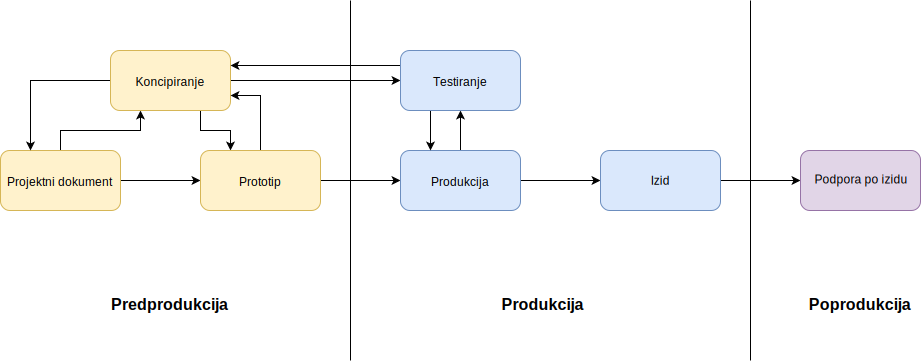
\includegraphics[width=15cm]{LifeCycle}
	\caption{Koraki razvoja igre}
	\label{slika:lifeCycle}
	\vspace*{-2em}
\end{figure}
\begin{enumerate}
	\item \textbf{Projektni dokument}. Tukaj preide ideja iz glave na fizični medij. Proces je zelo odvisen od velikosti projekta in studia. Pri večjih projektih nastane dejanski dokument, v katerem se definira ideja, kake bodo mehanike igre, zgodba, liki, razporeditev sredstev, predviden čas izdelave, ipd. Dokument je velikokrat tudi opremljen z konceptnimi slikami, ki jih pripravijo umetniki. S tem dokumentom je potem najlaže komunicirat vizijo preostalim ljudem v ekipi. Pri manjših idejah in posameznikih je ta korak bolj direkten. Ustvarijo se kake skice in krajši opisi, ampak večinoma pa se ta korak preskoči in je večji poudarek na prototipu.
	\item \textbf{Prototip}. Je najpomembnejši korak v procesu razvoja igre. Sama definicija pomeni razvoj osnovnega produkta, ki je ustvarjen z namenom testiranja koncepta \cite{blackwell2015prototype}. Glavni namen je preizkusit, ali je glavna ideja igre dovolj dobra, da iz nje nastane končni produkt. Prototipiranje je zelo povezano z samim koncipiranjem in projektnim dokumentom. Tukaj se identificirajo pomanjkljivosti, ki jih je potrebno razčistiti in mogoče znova koncipirati, ter prednosti, ki jih je potrebno poudariti v končnem produktu. Dober prototip je odličen mejnik v razvoju, ki se uporablja kot izhodiščna točka za začetek pravega projekta. Obenem služi kot prikaz koncepta možnim investitorjem, ki bi hoteli vložiti v projekt. 
	\item \textbf{Produkcija}. Je glavni del razvoja projekta. Sodelujejo vsi člani ekipe opisani v poglavju \ref{sec:opis_problema}. Konstantna komunikacija med razvijalci, preizkuševalci in oblikovalci pelje projekt skozi faze razvoja programske opreme: \textit{pre-alpha, alpha, beta, release candidate, live release (gold)}. Odvisno od projekta, se lahko studio odloči, da izdajo produkt končnim uporabnikom še v fazi razvoja. Tako postanejo uporabniki del preizkuševalcev, ki pomagajo pri razvoju projekta.
	\item \textbf{Izid}. Pomeni konec glavnega procesa razvoja. Igra se zapakira in distribuira do končnih uporabnik preko posrednikov. Ker mine kar nekaj časa od verzije, ki jo razvijalci dajo distribuiran na fizičnih medijih, do dejanskega izida, je danes ustaljena praksa prenos popravkov preko spleta na dan izida. Nekoč se je tukaj razvoj igre zaključil, razvijalci pa so prehajali na naslednji projekt. Dandanes pa izid pomeni le še en mejnik v samem življenjskem ciklu igre.
	\item \textbf{Podpora po izidu} . Tako imenovan \textit{post production} v angleščini postaja danes vedno večji faktor. Razvoj igre je veliki finančni podvig, ki največ sredstev terja do izida igre. Zato se veliki studii raje posvetijo izdani igri z nadaljnjo podporo. Začel se je uporabljati termin igre kot storitev (angl. \textit{games as a service}). Studii podpirajo igro še vrsto let z novimi vsebinami, popravki ter včasih korenitimi spremembami s ciljem maksimirati dobiček. Konstantna komunikacija z ciljno publiko je pomembna, saj tako identificirajo, kaj si igralci želijo novega v igri.
\end{enumerate}
Zgornji koraki so vidni v sliki \ref{slika:lifeCycle}. Kot vidno je proces razvoja, testiranja in koncipiranja zelo povezan, saj se igra konstantno izboljšuje.

\section{Marketing in viri občinstva}
Uspešna izdaja računalniške igre je zelo odvisna od marketinga pred izidom. Brez marketinga je zelo težko, da bo kdo našo igro opazil, kaj šele kupil. Samo na igralni platformi Steam letno izide več kot 6000 iger \cite{james6000Games}. V tej množici je pomembno, da naša igra izstopa in prav tukaj je zelo pomemben marketing že v zgodnjih fazah razvoja. Dober začetek marketinga je, ko lahko pokažemo glavne koncepte igre. Velikokrat so to slike ali videi igre v gibanju, ki pritegnejo končnega uporabnika \cite{robertMarketing}.

Obstaja veliko različnih načinov marketinga. Spodaj našteti so dandanes že skoraj obvezni, če hočemo uspeti na trgu \cite{robertMarketing}:
\begin{itemize}
	\item \textbf{Spletna stran.} Vsaka igra potrebuje svojo spletno stran. Brez le-te bo težko končna publika našla dodatne informacije o igri. Pomembno je, da stran vestno posodabljamo z opisom koncepta igre, slikami, videi, ipd. Ena možnost za hitro postavitev strani je \textit{presskit()} \footnote{http://dopresskit.com/}, prosto dostopen paket za enostavno stran za računalniško igro.
	\item \textbf{Blog.} Dober vir marketinga in občinstva je blog, kjer opisujemo potek razvoja igre. Veliko igralcev zanima, kako poteka razvoj in v katerem stanju se igra trenutno nahaja. Je tudi dober vir povezovanja z drugimi razvijalci, ki bi jih mogoče zanimalo sodelovanje na projektu. Paziti moramo le, da ne pretiravamo z objavami, saj ni vsak napredek v razvoju vreden omembe.
	\item \textbf{Socialni mediji.} Dandanes skoraj največja možnost pridobitve ciljnega občinstva so socialni mediji. Dobra stran igre na Facebook-u in kratke objave zanimive na Twitter-ju doprinesejo veliko. Socialna omrežja ponujajo tudi svoj plačljiv marketing s katerim lahko ciljamo specifično publiko, ki bi se zanimala za našo igro.
	\item \textbf{Konference.} Vsako leto poteka več konferenc, kjer se razvijalci predstavijo s svojimi igrami. Na konferenci se obrne veliko igralcev in različnih medijev, ki zelo pripomorejo k marketingu igre. Tri izmed večjih takih konferenc so Pax\footnote{http://www.paxsite.com/}, IndieCade\footnote{http://www.indiecade.com/} in Indie Mega Booth\footnote{http://indiemegabooth.com/}. V Sloveniji je največja konferenca SGC\footnote{http://sgc.si/}.
	\item \textbf{Množično financiranje (angl. crowdfunding).} Danes vedno bolj popularen način zbiranja sredstev in občinstva za razvoj igre. Preko strani kot je Kickstarter predstavimo svojo vizijo in načrt razvoja, ter tako poskusimo doseči igralce, ki bi jih zanimala naša igra. Ti pa lahko nato financirajo razvoj.
	\item \textbf{Napovednik (angl. trailer).} Ko se igra začne bližati zaključnim fazam razvoja je dobro izdelati napovednik, ki se bo potem uporabil na platformah, kjer bomo igro izdali. V napovedniku je pomembno, da prikažemo glavni koncept igre in da smo iskreni. Zavajajoči napovedniki lahko ustvarijo večjo začetno zanimanje vendar po izidu hitro pritegne slabo kritiko.
\end{itemize}

\section{Možnosti izdaje igre}
Opisali smo nekaj možnosti, ki so nam na voljo za izdajo igre kot individualnemu razvijalcu. Večina teh možnosti predvideva, da nimamo svojega distributerja in so zato najbolj primerne za manjše projekte:
\begin{itemize}
	\item \textbf{Steam.} Največja platforma za digitalno distribucijo računalniških iger. Omogoča izgradnje svoje strani za našo igro z vsemi potrebnimi informacijami. Sama platforma poskrbi za distribucijo, namestitev, posodobitve, varnostno kopijo shranjenih iger, glasovno komunikacijo v igri ipd. Na voljo je na vseh večjih operacijskih sistemih kot so Windows, OSX in Linux. Če se odločimo, da bomo našo igro izdali na Steam platformi, nam Steam ponudi implementacijo njihovega SDK, ki nudi proti-piratsko rešitev, mikro transakcije, oblačne storitve, dosežke ipd. Cena za izdajo igre je 100 evrov, provizija za vsako prodano kopijo igre pa je 30\% \cite{steam}.
	\item \textbf{Itch.io.} Zelo popularna rešitev za individualne razvijalce, saj ne stane nič, da svojo igro dodamo na njihovo platformo. Podobno kot Steam ponujajo izgradnjo svoje strani za igro ter aplikacijo, ki skrbi za namestitve in posodobitve. Platforma ne ponuja svoj SDK, ki bi nudil dodatne funkcionalnosti. Možno je nastaviti minimalno ceno igro, kupci pa lahko po želji plačajo več. Provizija je 10\% od vsakega nakupa, po želji pa lahko povečamo ta delež \cite{itchiofaq}.
	\item \textbf{Humble Bundle.} Ponuja tri vrste prodaje skozi njihovo platformo. Prva možnost je izgradnja zastonj strani, kjer ponujamo svojo igro. Oni poskrbijo za transakcije in si vzamejo 5\% provizije. Ta stran je neodvisna od njihove trgovine. Druga možnost je samostojen majhen gradnik, ki ga potem lahko dodamo na svojo spletno stran. Podobno kot pri njihovi neodvisni strani si vzamejo 5\% provizije. Zadnja možnost pa je prodajanje na njihovi spletni trgovini. Tukaj lahko dobimo njihovo izpostavitev naše igre, imamo znižanja ipd. So samo spletna trgovina, ne ponujajo aplikacije za prenašanje in posodabljanje iger. Provizija za prodajo v njihovi trgovini je 25\%, ne stane pa nič, da svojo igro objavimo \cite{humblebundle}.
	\item \textbf{GameJolt.} Podobno kot itch.io je zelo popularna platforma za neodvisne razvijalce. Nudijo svojo aplikacijo za prenose in posodobitve. Objava igre v njihovo trgovino ne stane nič, provizija pa je 10\% ali manj saj ponujajo možnost znižanja provizije. Promovirajo skupnost neodvisnih razvijalcev, zato vse dobičke dobimo na njihov račun, ki jih lahko nato porabimo za nakup iger drugih razvijalcev, brez dodatne provizije. Seveda je možno denar si vedno izplačati \cite{gamejolt}.
	\item \textbf{Apple store in Google Play.} Če je naša igra namenjena za mobilne naprave, potem moramo obvezno uporabiti ti dve trgovini. Obe nudita izgradnjo svoje strani za igro na trgovini, prenose, posodobitve in dodatne transakcije. Kot mobilna platforma ponujata tudi dodatni SDK, s katerimi lahko v našo igro vgradimo lestvice, nagrade, oblačne storitve ipd. Provizija je 30\% od nakupa, je pa potrebno tudi plačati za objavo aplikacije v trgovini. Pri Google Play je to enkratna cena 25 evrov, nakar lahko izdajamo koliko hočemo aplikacij \cite{googleplay}. Pri Apple store je cena 99 evrov na leto \cite{applestore}.
\end{itemize} 

\chapter{Orodja za izdelavo iger}\thispagestyle{fancy}
\section{Načrtovanje in vodenje razvoja}
Dobra organizacija veliko prispeva za tekoč razvoj računalniške igre. Obstaja veliko različnih orodij, nekatere so usmerjene za organizacijo ljudi in opravil, druge za organizacijo projekta in kode. Tudi, če samostojno razvijamo igro nam ta orodja veliko pomagajo, zato smo poiskali dobre rešitve in jih tudi opisali.

\subsection{Organizacija ljudi in opravil}
Delo je priporočljivo razdeliti na manjša opravila, ki jih lahko opišemo, razdelimo med skupino in vodimo njihov napredek. Dve izmed boljših orodij za to sta Trello in HackNPlan. Obe pa uporabljata principe kanban razvojnega sistema.

\begin{figure}[h]
	\centering
	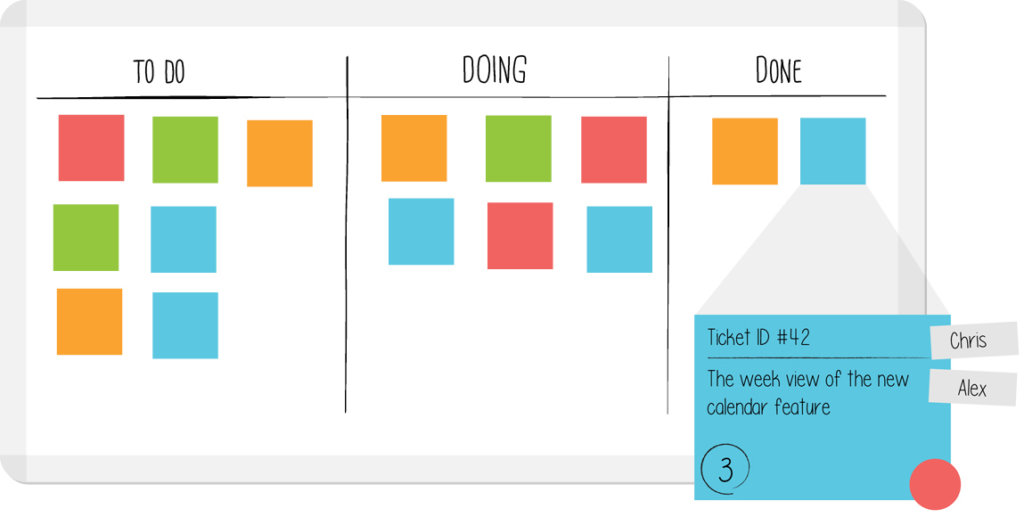
\includegraphics[width=10cm]{kanban_guide_print_KPO_bleed_board2}
	\caption{Kanban tabla. Vir \cite{kanbanBoard}}.
	\label{slika:kanbanBoard}
	\vspace*{-2em}
\end{figure}

Kanban sistem je način organizacije dela, katerega cilj je izboljšati ravnovesje med povpraševanjem in kapaciteto človeškega dela, ki je na voljo. Delo je razdeljeno na manjše kose in vizualizirano na kanban tabli kot primer na sliki \ref{slika:kanbanBoard}. Opravila so večinoma vizualizirana na listkih, ki hranijo potrebne podatke kot so naslov, opis, ocenjen čas potrebnega dela, trenutni upravitelji ipd. Ta opravila so uvrščena na pripadajoč del table, odvisno v kakem stanju je opravilo (npr. čaka na dela, v razvoju, v testiranju, potrebno ocene, končano, ipd.). Glavni cilj take organizacije je vizualizirati in kategorizirati opravila, ki jih nato razvijalci prevzamejo in opravijo \cite{kanbanBoard}.

Trello je produkt pod okriljem podjetja Atlassian, ki med drugim nudijo storitve kot so Jira in BitBucket. Ponuja nam izgradnjo tabel, na katera dodajamo opravila v obliki kartic z vsemi potrebnimi informacijami. Razvijalce lahko razvrstimo v skupine in tabele, nakar se lahko dodelijo na opravilo. Primer demo table je viden na sliki \ref{slika:trelloDemo}. Storitev je na voljo preko spletne strani, ponujajo pa tudi mobilno aplikacijo. Vsa funkcionalnost je na voljo zastonj, z možnostjo nadgradnje za 9.99 dolarjev za vsakega člana na mesec. Nadgradnja nam omogoči nalaganje večjih datotek, dodatne varnostne funkcionalnosti, prvo ročno pomoč od podjetja ter več integracij za vsako tablo. Integracije so na voljo z njihovimi in drugimi produkti za lažjo organizacijo. Zastonjska verzija je za individualni razvoj več kot dovolj, saj so nadgradnje namenjene za večje projekte in skupine.

\begin{figure}[h]
	\centering
	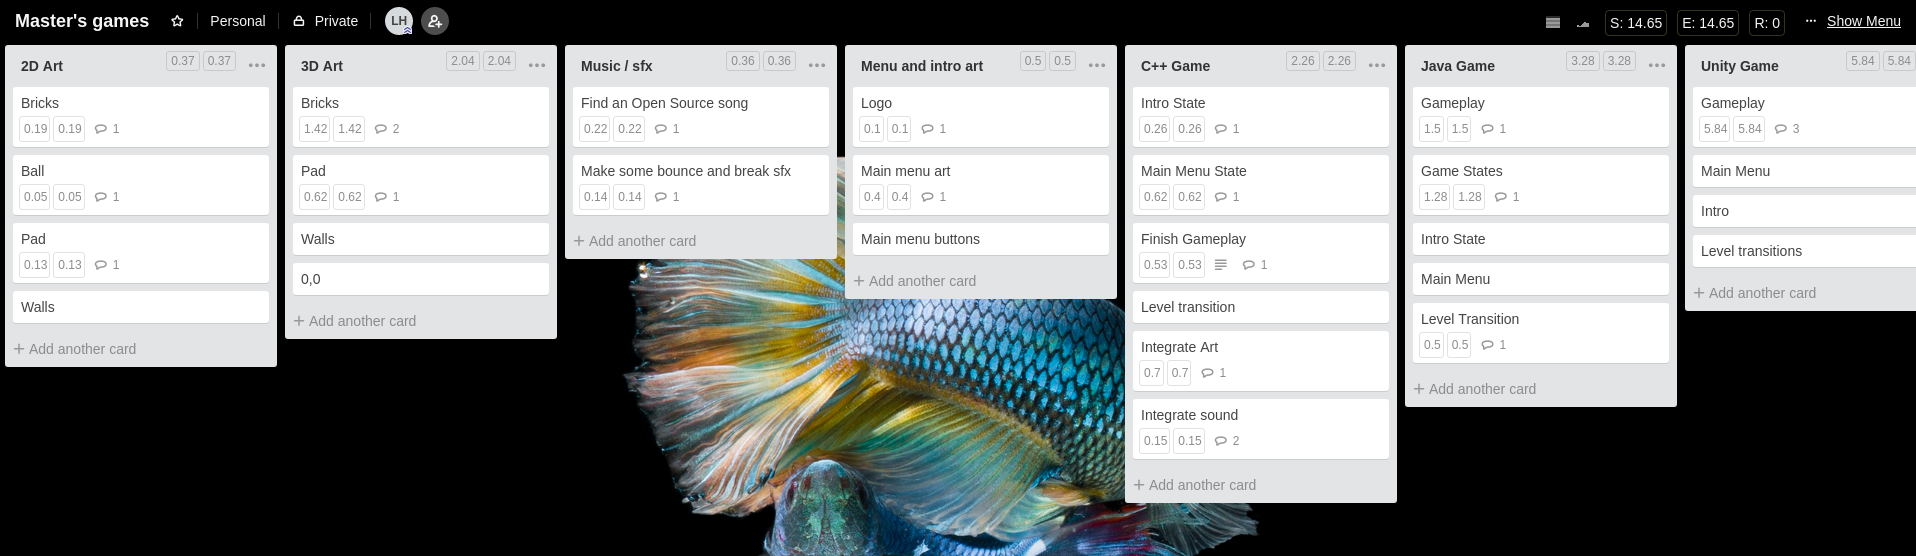
\includegraphics[width=10cm]{trelloBoardDemo}
	\caption{Primer Trello table.}.
	\label{slika:trelloDemo}
	\vspace*{-2em}
\end{figure}

HackNPlan je v osnovi podoben kot Trello, vendar je zgrajen specifično za razvoj računalniških iger. Poleg kanban table in organizacije ljudi ponuja še preglede statistik, vodenje sprintov ter funkcionalnost za skupno koncipiranje in dokumentiranje idej. Primer table vidimo na sliki \ref{slika:hacknplanDemo}. Vso našteto funkcionalnost dobimo v zastonjski verziji ponujajo pa tudi nadgradnjo za dodatne storitve. Cena nadgradnje je 4 evre na mesec in glavna dodatna funkcionalnost so integracije z drugimi storitvami kot so GitHub, Slack, ipd. Zastonjskih integracij ni, zato je na tem področju slabši produkt kot Trello, vendar pa specifične funkcionalnost za namen razvoja iger veliko pripomorejo.

\begin{figure}[h]
	\centering
	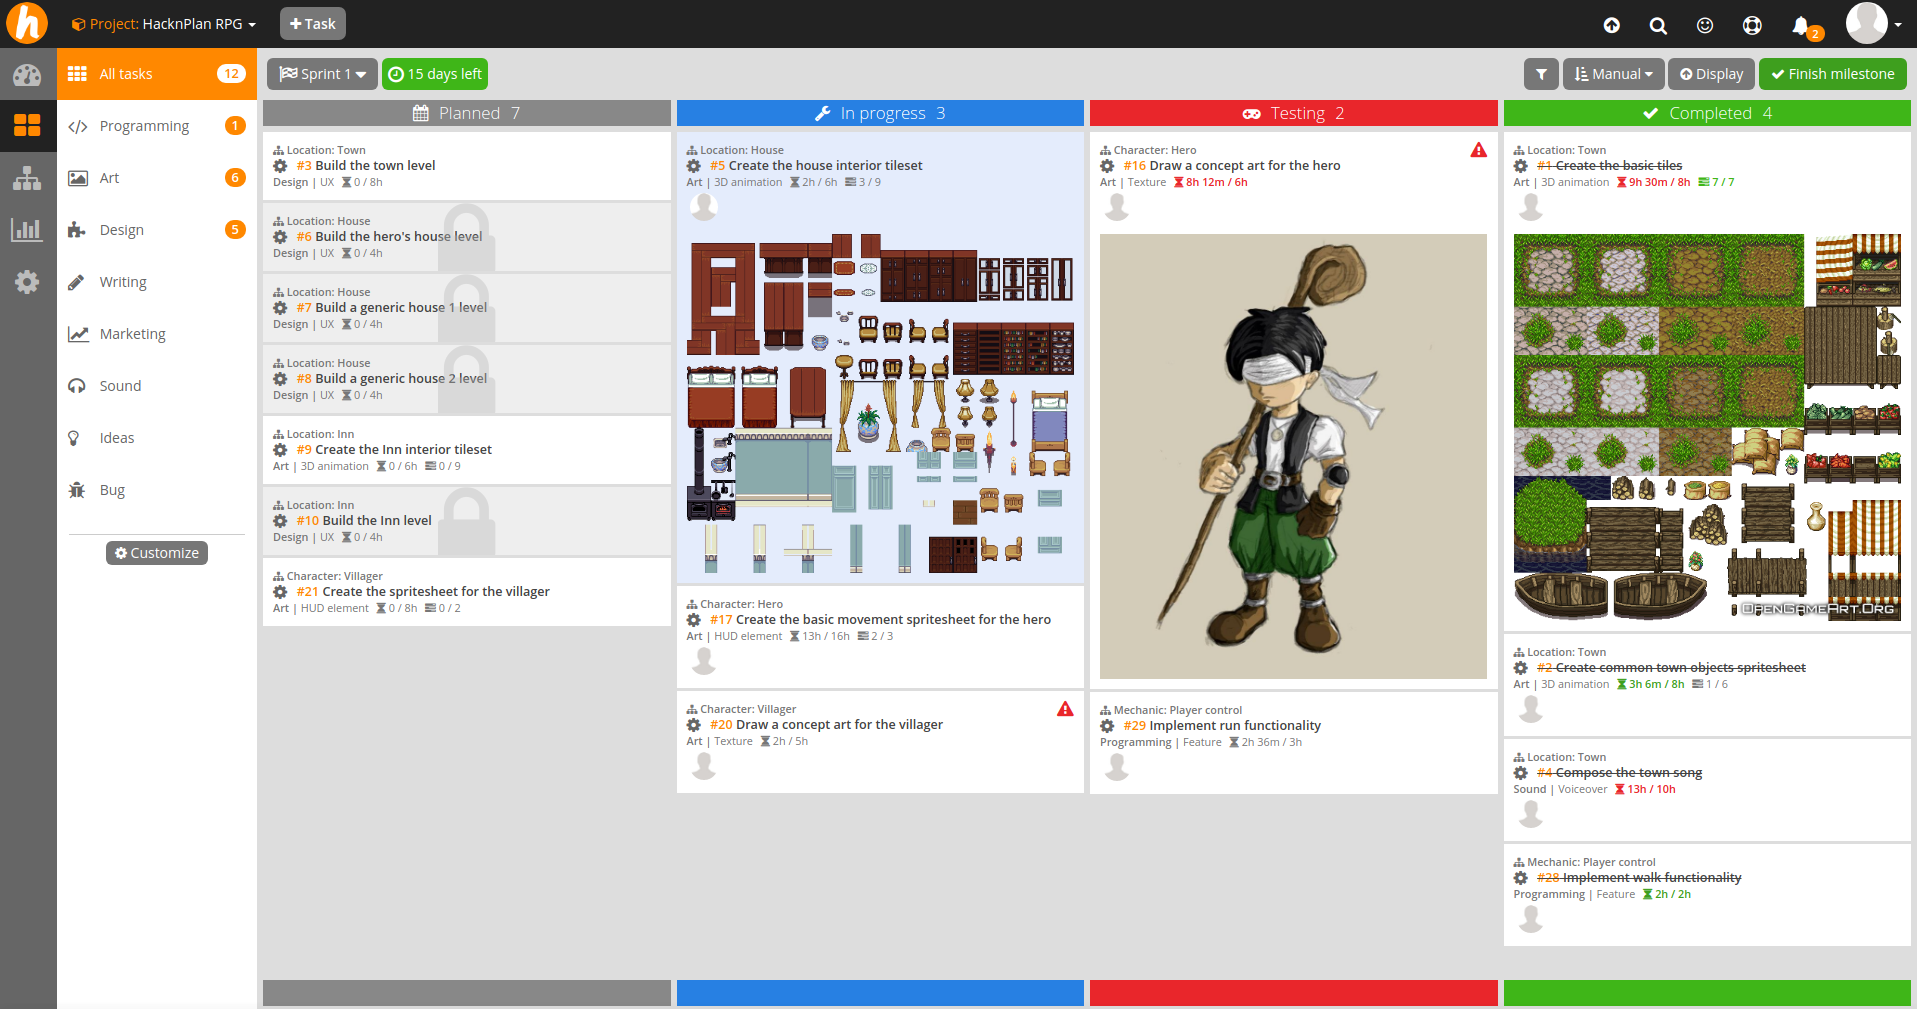
\includegraphics[width=13cm]{hacknplanDemo}
	\caption{Primer HackNPlan table.}.
	\label{slika:hacknplanDemo}
	\vspace*{-2em}
\end{figure}

\subsection{Organizacija projekta in kode}
Enako pomembno kot organizacija opravil je organizacija samega projekta med razvojem. Za te potrebe obstaja več rešitev verzioniranja projektov kot so SVN, Mercurial, GIT, Perforce, itd. Te programske rešitve ponujajo način hranjenja trenutnega stanja projekte kode na centralnem mestu, obenem pa sledijo vsem spremembam vsake datoteke. Mogoče je tudi hraniti več različnih aktualnih verzij iste datoteke v različnih vejah, in jih nato združiti v končno obliko. Vsak razvijalec ima lokalno svojo kopijo projekta in svoje spremembe pošilja v centralni repozitorij. Tako v ozadju nastaja drevesna struktura sprememb projekta skozi čas. Primer takega grafa vidimo na sliki \ref{slika:gitGraph}. Vsaka sprememba je komentirana s strani razvijalca in tako je možno hitro poiskati in preiti na starejšo verzijo v primeru težav \cite{versionControl}.
	
\begin{figure}[h]
	\centering
	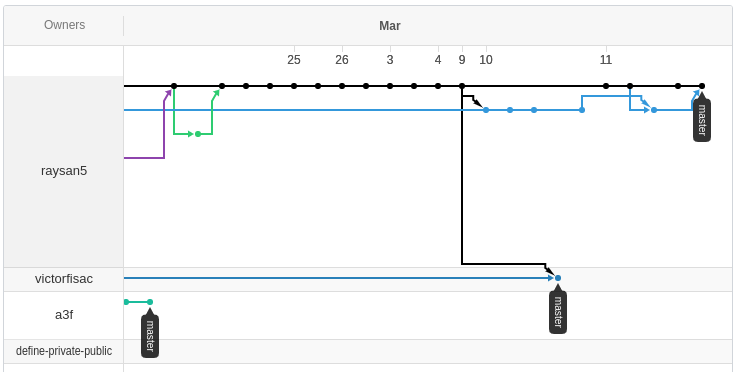
\includegraphics[width=13cm]{gitGraph}
	\caption{Primer grafa sprememb Raylib projekta na GitHub-u.}.
	\label{slika:gitGraph}
	\vspace*{-2em}
\end{figure}

V industriji razvoja računalniških iger je najbolj uporabljen sistem verzioniranja Perforce, saj deluje najboljše za večje projekte in kot komercialna plačljiva programska rešitve ponuja zelo močna orodja za delo z binarnimi datoteka (umetniški in zvočni gradniki so velikokrat v binarnem formatu in obenem največje datoteke v projektu). Za večje projekte je Perforce plačljiv, ponujajo pa zastonjsko različico za projekte do 5 ljudi.

Najbolj preprost za uporabo in najbolj razširjen pri razvoju programske opreme pa je sistem Git. Popularnost je v veliki meri povezana s storitvijo GitHub, ki ponuja oblačno hranjenje repozitorija z našim projektom, obenem pa nudi funkcionalnost za lažje skupno delo na projektu. Alternativa GitHub-u je BitBucket, obe rešitvi pa smo analizirali za potrebe razvoja igre.

GitHub je spletna platforma zgrajena na bazi sistema verzioniranja Git. Glavna storitev je gostovanje našega repozitorja v oblaku, vendar imajo še obilo drugih storitev zaradi česar so zelo priljubljeni za veliko projektov. Omogočajo upravljanje z ljudmi in skupina, kdo ima dostop do kode, kdo dela na čem ipd. Pregled sprememb je preprost za uporabo in omogoča komentiranje nad kodo. Za vsak projekt nudijo tudi sistem sledenju napak (npr. kot Bugzilla), kjer lahko vsi, ki uporabljajo programsko opremo javijo napake in komunicirajo z razvijalci. Zelo popularna funkcionalnost so tudi zahteve za spremembe (angleško \textit{pull request}), kjer lahko nekdo izdela in predlaga spremembe za projekt, nato pa se razvijalci odločijo, ali bodo te spremembe integrirali v glavno vejo projekta. Za odprtokodne in javne projekte je vsa za funkcionalnost zelo dobrodošla, saj nudi lažje upravljanje z projektom. Zastonjska verzija Github-a ponuja vso našteto funkcionalnost, omejitev je le v tem, da morajo vsi naši projekti biti javni. Če hočemo imeti zasebni projekt na Github, potem je potrebno plačat 7 evrov mesečno \cite{github}.

Alternativa Github-u je storitev BitBucket. Ponuja enako funkcionalnost vendar v zastonjski storitvi dovolijo zasebne repozitorije. Omejitev zastonjskega paketa je maksimalno 5 razvijalcev na projektu. Če hočemo povečati število razvijalcev je cena 2 evra na razvijalca na mesec. Za projekte z manjšo skupino je torej BitBucket boljša rešitev za privatni repozitorij. Če pa hočemo, da je naš projekt na voljo vsem, je pa boljša alternativa GitHub \cite{bitBucket}.

\section{Orodja za izdelavo grafičnih gradnikov}
Grafični gradniki so pri razvoju računalniške igre uporabljeni od samega koncipiranja do končnega izida igre. Mi smo se osredotočili na gradnike, ki se uporabijo v sami računalniški igri. Ti gradniki so odvisno od tipa igra 2D slike ali 3D modeli. Na trgu obstaja veliko rešitev za izdelavo teh gradnikov, mi pa smo analizirali zastonjsko programsko opremo, ki ima več kot dovolj funkcionalnosti za izdelavo potrebnih gradnikov za individualne projekte.

\subsection{2D grafični gradniki}
Individualni projekti večinoma uporabljajo dva stila 2D grafičnih gradnikov. Angleško imenovana \textit{pixel art} in \textit{vector art} (slovensko vektorska umetnost). Končni rezultat je kljub imen vedno rastrska slika, razlika je kako so gradniki ustvarjeni in kaj je v stilu pomembno. Pixel art izhaja iz navdiha iz starih igralnih sistemov, kjer so bile omejitve v smislu resolucije gradnikov in razpoložljivosti barv. Pomembno je izkoristiti vsak piksel, ki je na voljo. Vektorski gradniki pa v nasprotju ciljajo na gradnike višje resolucije. Poskušajo uporabiti preproste oblike in združevanje le-teh za pridobitev končnih slik. Razliko v stilih vidimo na sliki \ref{slika:pixelVsVector}.

\begin{figure}[h]
	\centering
	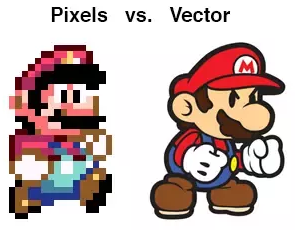
\includegraphics[width=6cm]{pixelVsVector}
	\caption{Razlika v stilih 2d grafičnih gradnikov. Vir \cite{pixelVsVector}}
	\label{slika:pixelVsVector}
\end{figure}

Program, ki ga priporočamo za izdelavo 2D pixel art gradnikov je Aseprite\footnote{https://www.aseprite.org/}. Vsa potrebna funkcionalnost za delo z slikami iz profesionalnih programov je na voljo, vendar so vse prilagojene za delo s slikami nižjih resolucij. Zelo močna so tudi orodja za delo z animacijami, plastmi, ipd. Za namen razvoja računalniških iger nam ponuja tudi posebne izvoze v teksturne atlase in nize slik za animacijo. Program je na voljo za 15 evrov, vendar je vsa izvorna koda javna. Uradno da si lahko sami zgradimo program in ga uporabljamo v komercialne namene. Prednost plačljive različice so samodejne posodobitve, ni potrebno prevajati izvorne kode ter seveda podpora nadaljnjega razvoja.

Za razvoj vektorske grafike pa predlagamo program Inkscape\footnote{https://inkscape.org/en/}. Po funkcionalnost je podoben Adobe Illustrator-ju, le da je na voljo kot zastonjska odprtokodna rešitev. Manjkajo napredne funkcionalnosti koz je zvijanje združenih objektov za potrebe animacije, vendar na trgu ni boljše zastonjske alternative. V Inkscape delamo z vsemi liki kot z objekti, in nad njimi lahko izvajamo booleanove transformacije (presek, unija, odštevanje, ipd.) ter tako ustvarimo željene like. Ker delamo z objekti je naš končni izdelek neodvisen on resolucije in ga lahko izvozimo v željeni velikosti za našo igro. 

\subsection{3D grafični gradniki}
Izdelava 3D modelov je bolj zahtevna od 2D gradnikov saj je potrebnih več korakov (modeliranje, teksture, animiranje). V industriji se uporabljajo različni programski paketi kot so Maya, Houdini, ZBrush in Blender\footnote{https://www.blender.org/}. Od teh je Blender edini zastonjski in odprtokodni program, ki je na voljo na vseh operacijskih sistemih. V zadnjih letih je vedno bolj uporabljen v industriji, saj se s svojo funkcionalnostjo lahko kosa z drugimi plačljivimi programi in jih na določenih mestih celo preseže. Primer programa vidimo v sliki \ref{slika:blenderDemo}.

\begin{figure}[h]
	\centering
	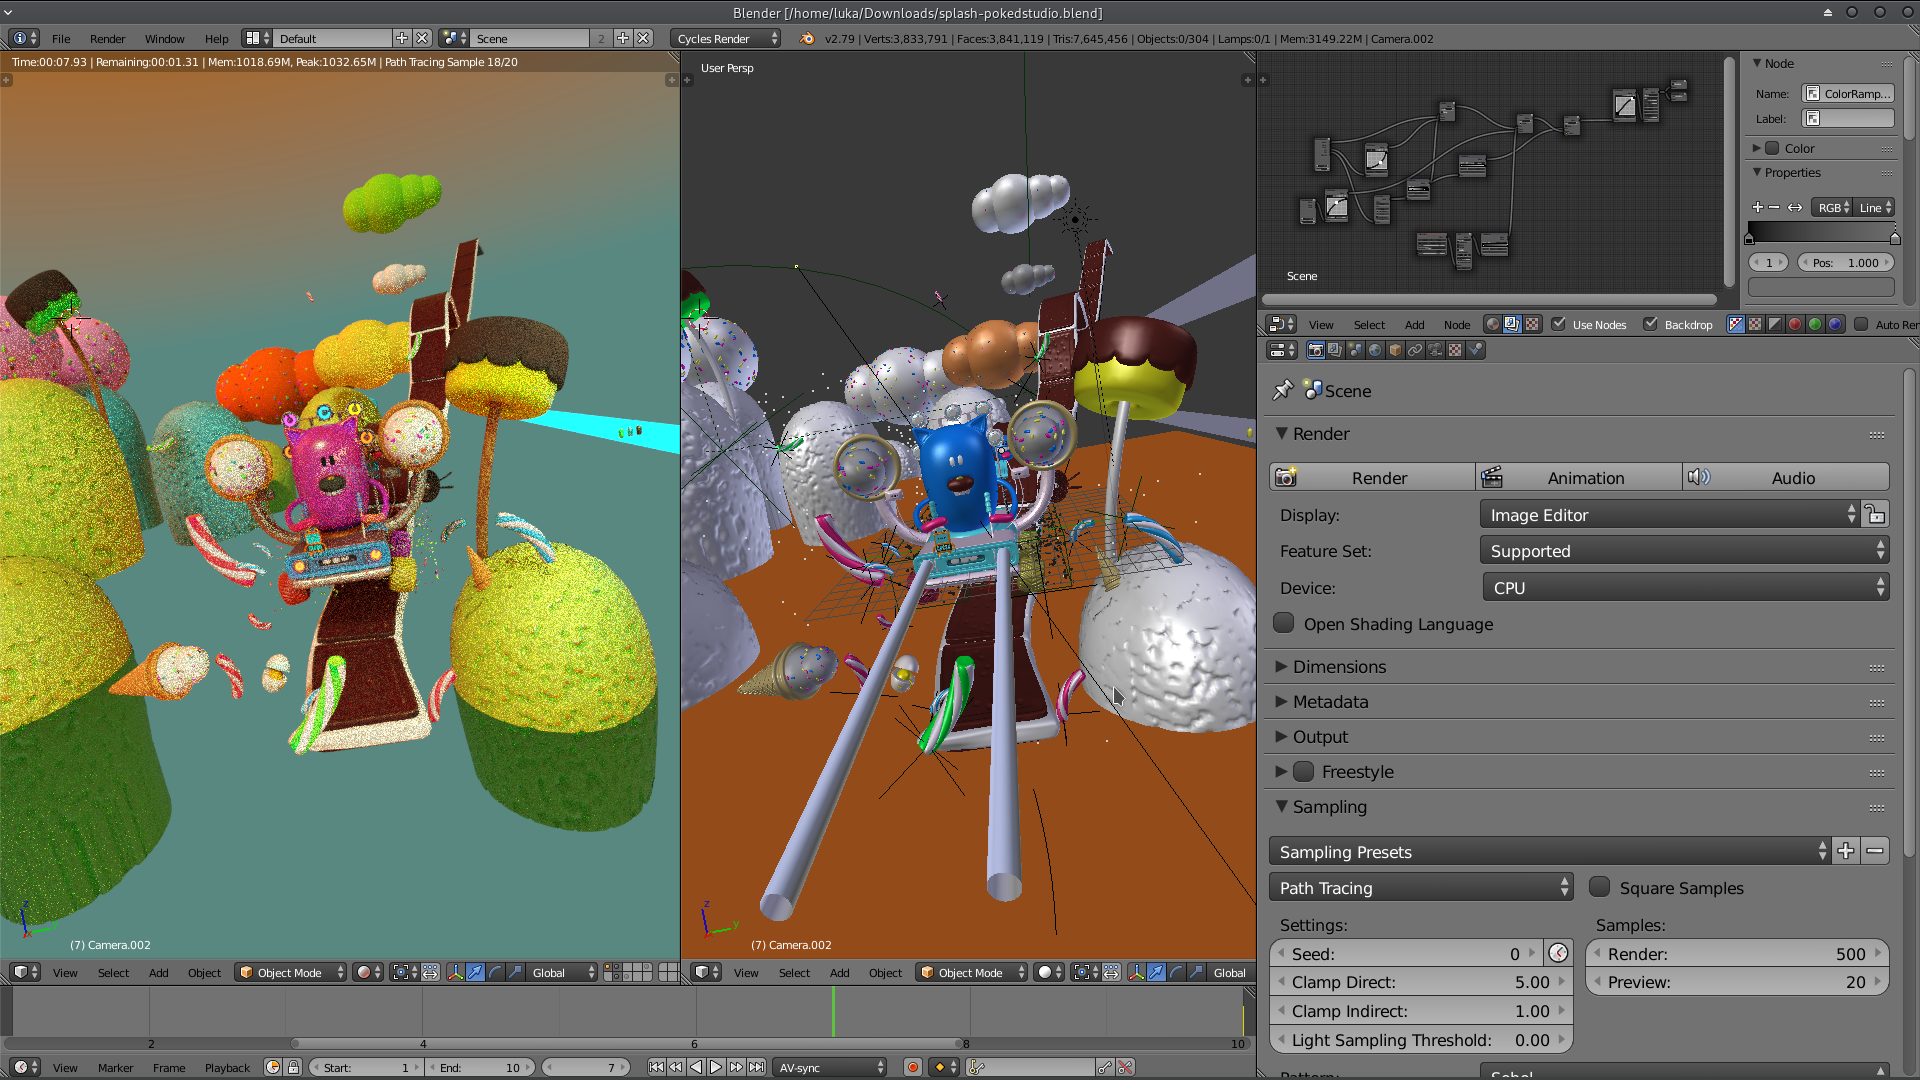
\includegraphics[width=13cm]{blenderDemo}
	\caption{Blender programski paket}
	\label{slika:blenderDemo}
\end{figure}

\section{Orodja za izdelavo zvočnih gradnikov in glasbe}
Za izdelavo zvočnih gradnikov (oziroma efektov v nadaljevanju) smo podobno kot pri izdelavi grafičnih gradnikov analizirali zastonjske rešitve, ki ponujajo potrebne funkcionalnosti za razvoj. Glavna ločitev med zvočnimi efekti in glasbo je, da se efekti uporabljajo za različne akcije v igri (npr. streli orožij, skok, šumenje, ipd.), nakar primerna glasba pa igra v ozadju glede na trenutno splošno dogajanje. Velikokrat se uporabljajo namenski programi za izdelavo glasbe tudi za izdelavo efektov, vendar obstaja nekaj orodij, ki so namenjene specifično za to.

Izdelava zvočnih efektov ima dva pristopa. Za bolj kvalitetne efekte se v studijo posnamejo dejanski zvoki, ki bi bili primerni za igro. Recimo za strele orožij se posnamejo streli avtentičnih orožij, šumenje se simulira z listjem ipd. Ti zvoki se potem obdelajo in prilagodijo v programski opremi za delo z zvokom/glasbo. Drugi način je generiranje zvokov iz računalniško ustvarjenih zvokov in šumov. Z uporabo različnih valovnih oblik (sinusoida, trikotni val, rampa, kvadrat, ipd.), filtrov in različnih modulacij ustvarimo željene efekte. Namenski programi za ta proces so Bfxr, Labchirp, DSP Retro/Anime, ipd. Labchirp in DSP delujeta le na platformi Windows, obenem je DSP plačljiv, zato smo za analizo izbrali Bfxr\footnote{https://www.bfxr.net/}, ki je prosto dostopen in obenem uporaben kar s spleta. Program vidimo na sliki \ref{slika:bfxr}. Kot je z slike razvidno, imamo možnost izbire različnih valovnih funkcij, ki jo nato spreminjamo s ponujenimi drsniki. Ustvarjene efekte lahko tudi združimo skupaj in na koncu izvozimo v Wav formatu za uporabo v igri.

\begin{figure}[h]
	\centering
	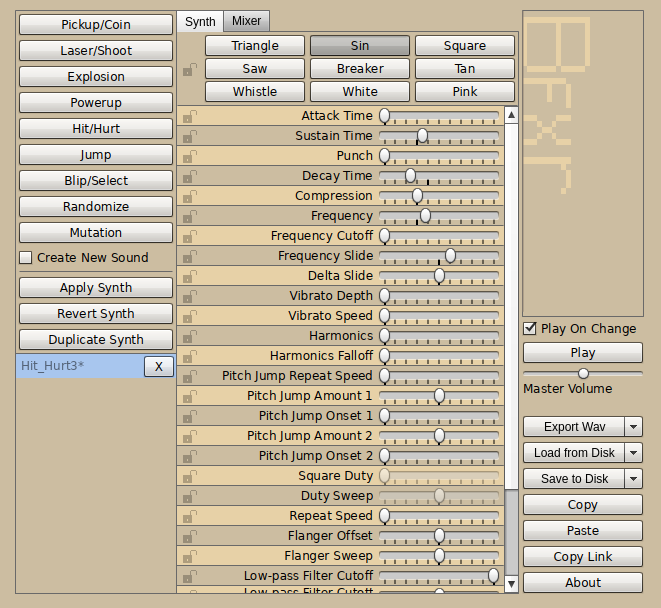
\includegraphics[width=10cm]{bfxr}
	\caption{Program Bfxr}
	\label{slika:bfxr}
\end{figure}

Izdelava glasbe je bolj pokrita z programskimi paketi kot izdelava efektov. Med bolj znane sodijo FL Studio, Reaper, Logic Pro X, itd. Vsi našteti so plačljivi z minimalno vstopno ceno vsaj 100 evrov. Obstaja tudi nekaj prosto dostopnih rešitev kot so Ardour in LMMS\footnote{https://lmms.io/}, ki smo ga bolj podrobno analizirali. Je odprto kodni program in je na voljo na vseh operacijskih sistemih (Windows, Linux, OS X). Na sliki \ref{slika:lmms} vidimo primer izdelave skladbe. Izberemo si različne inštrumente (na voljo so godala, tolkala, pihala, klaviature, možno si je tudi ustvariti sintetično glasbilo) in z njimi ustvarimo vse potrebne dele skladbe s postavljanjem posameznih not. S tem ustvarimo sekcije, ki jih nato sestavljamo v končni produkt.

\begin{figure}[h]
	\centering
	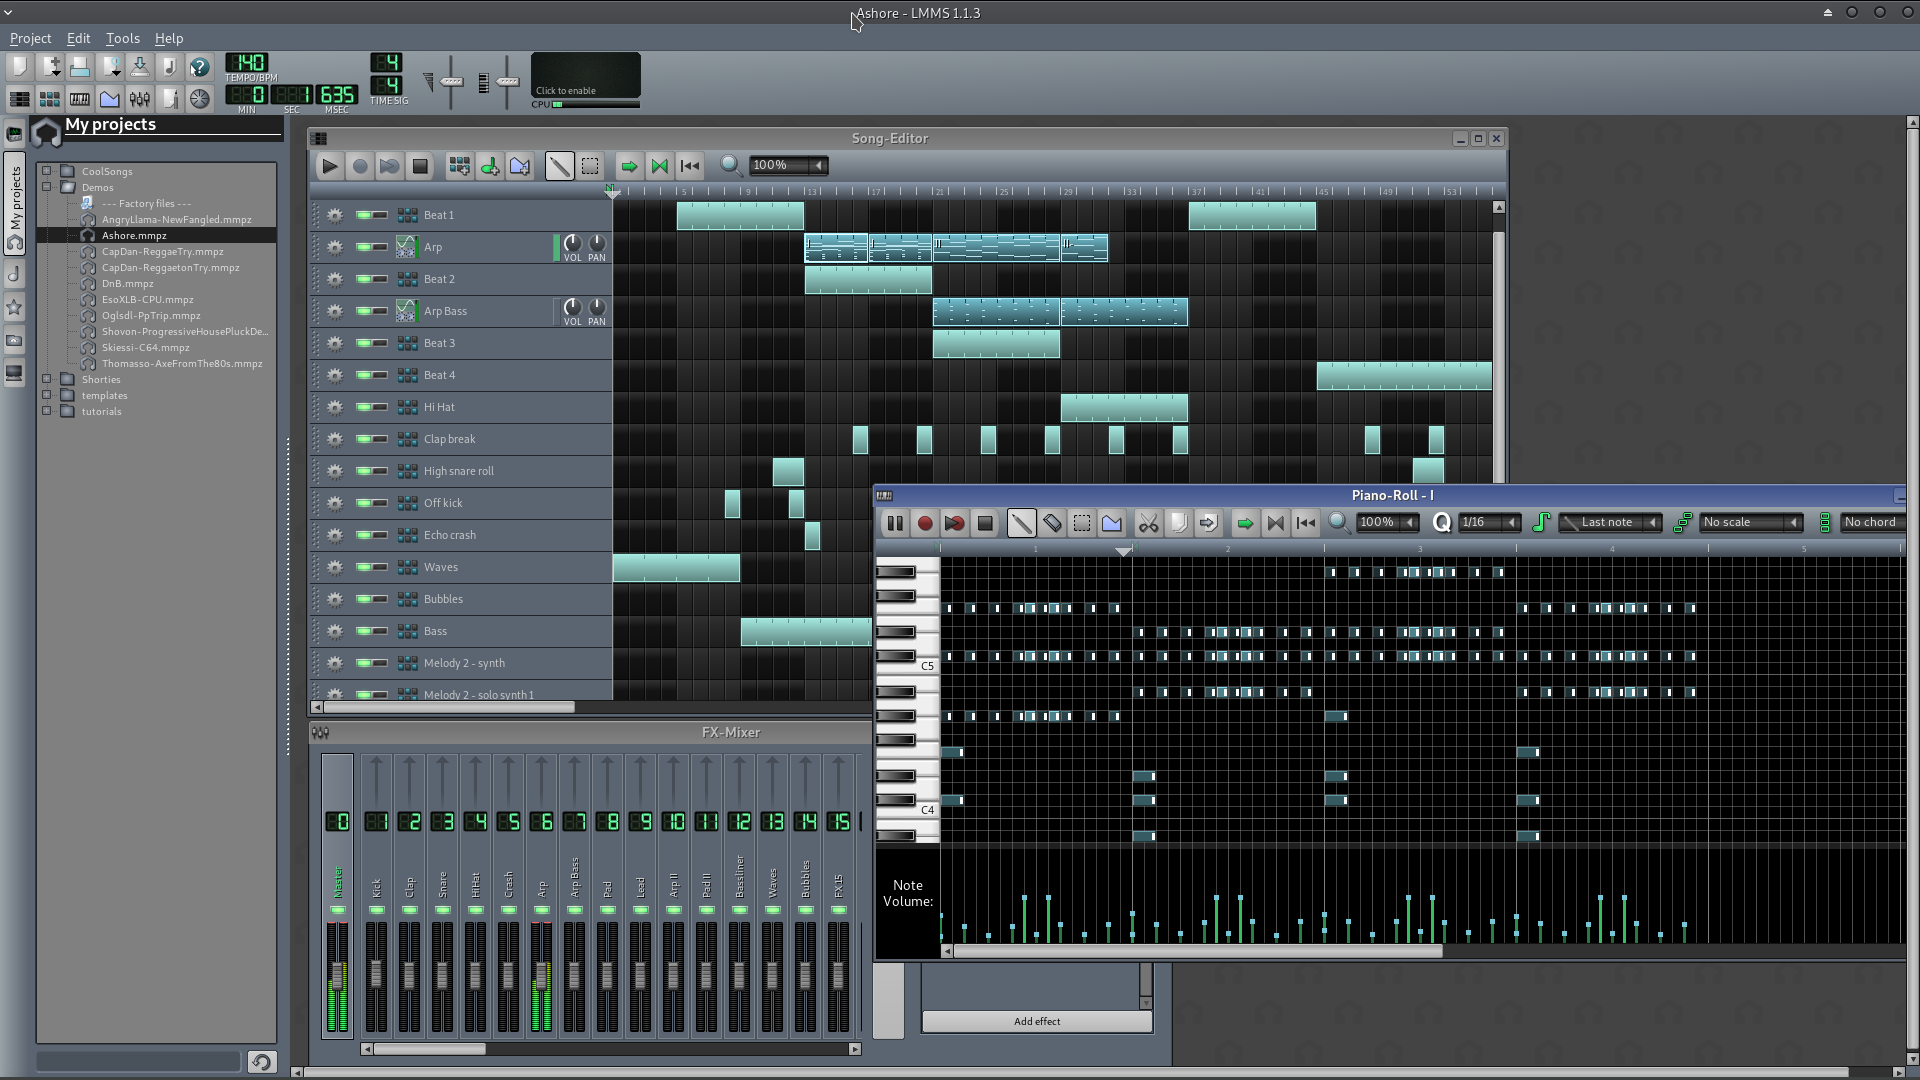
\includegraphics[width=12cm]{lmms}
	\caption{Program LMMS med izdelavo skladbe}
	\label{slika:lmms}
\end{figure}

\section{Računalniške knjižnice, ogrodja in pogoni}
Glavni cilj magistrske naloge je uporabiti in opisati orodja za tehnično implementacijo računalniške igre. Tehnično implementacijo mislimo kot samo programiranje oziroma razvoj igre. Zato smo raziskali in opisali različna orodja, ki so nam na voljo v tem poglavju, njihovo uporabo in prakse pa sledijo v poglavju \ref{chapter:razvojIger}. Omejili smo se na orodja, ki so na voljo na vseh večji operacijskih sistemih (Windows, Linux in OS X) in je z njimi možno izdelati računalniško igro za vse tri sisteme (po možnosti tudi več npr. mobilne in spletne platforme).

Tehnično implementacijo računalniške igre smo v našem delu kategorizirali v tri različne smernice: nizkonivojske knjižnice, visokonivojske knjižnice in ogrodja ter namenske pogone.

\subsection{Nizkonivojske knjižnice}
V to kategorijo smo uvrstili knjižnice, ki nudijo specifičen nabor funkcionalnosti potrebne za razvoj računalniške igre. Omejili smo se na programski jezik C++, saj je najbolj razširjen v industriji razvoja iger. Te knjižnice pokrivajo eno ali več izmed naslednji funkcionalnosti: upravljanja z okni, vhodni sistemi (tipkovnica, miška, igralni ploščki, ipd.), računalniška grafika, predvajanje zvoka, medmrežna komunikacija, matematične funkcije, fizikalni pogoni, itd. Težko je definirati mejo med knjižnico in ogrodjem (angleško \textit{framework}), vendar v splošnem knjižnice v tej kategoriji ne pokrivajo vse potrebne funkcionalnosti za razvoj. Potrebno je uporabiti kombinacijo le-teh, da uresničimo končni projekt.

Najprej je potrebna osnovna knjižnica, ki ponuja osnovno funkcionalnost za vzpostavitev programa. Sem spadata knjižnici SDL\footnote{https://www.libsdl.org/}\cite{sdllib} in GLFW\footnote{http://www.glfw.org/}\cite{glfw}. Obe ponujata abstrakcijo za potrebno delo z okni na namizju, dostop do vhodnih naprav, kontekst za upravljanje z grafičnim cevovodom kot je OpenGL, Direct3D ali Vulkan, ipd. Sta temelj večini iger, ki se razvijajo z nizkonivojskimi knjižnicami, obenem pa sta tudi izhodiščna točka za namenske pogone kot je Source Engine \cite{sourceEngineSDL} in Cryengine \cite{cryengineSDL}.

Preden nadaljujemo je potrebno omeniti še grafične cevovode. Tukaj obstajajo trenutno trije standardi: Direct3D, OpenGL in Vulkan. Direct3D je član paketa DirectX, skupek knjižnic za razvoj računalniških iger od podjetja Microsoft. Podobno kot SDL ponuja DirectX paket vseh potrebnih funkcionalnosti za razvoj, vendar je na voljo samo za Windows platformo in igralno konzolo Xbox. Zato nismo opisali grafičnega cevovoda Direct3D, saj ni na voljo za vse platforme. OpenGL in Vulkan pa sta standarda za delo z grafičnim cevovodom, razvoj nad njima vodi konzorcij Khronos Group. OpenGL so začeli razvijati leta 1992, Vulkan pa je nekako naslednik tega standarda, z začetkom razvoja leta 2016. Oba standarda ponujata način dela z grafičnimi karticami, za potrebe izrisovanja 2D in 3D grafike. Oba standarda imata svoje knjižnice, ki za delo potrebujejo samo kontekst do grafične kartice, ki ga ponudi osnovna knjižnica kot je SDL ali GLFW \cite{opengl}. 

SDL ponuja še razširitve v obliki dodatnih knjižnic za dostop do specifične funkcionalnosti:
\begin{itemize}
	\item \textbf{SDL\_Image}. SDL v osnovi ponuja podporo za omejeno število slikovnih formatov. Če hočemo prebrati druge formate potrebujemo dodatno knjižnico. SDL\_Image ponuja podporo za popularne formate BMP, GIF, JPEG, PNG, SVG in še druge. Obenem so funkcije pripravljene tako, da je lažje uporabljati te slike v kontekstu SDL knjižnice, kot pa če bi uporabljali katero bolj splošno knjižnico za slike kot je SOIL \cite{sdlimage}.
	\item \textbf{SDL\_Mixer}. Osnovna SDL knjižnica podpira nalaganje glasbenih datotek v formatu WAV. Obenem je možno predvajati zvoke po samo enem kanalu naenkrat kar pomeni, da ne moremo predvajati več različnih efektov naenkrat, brez da bi sami spisali algoritem za mešanje efektov. Zato ponujajo razširitveno knjižnico SDL\_Mixer, ki odpravi te omejitve. Doda podporo za branje datotek formata FLAC, OGG, MP3, MOD in MIDI. Obenem ponuja prevajanje zvokov po več različnih kanali. Tako lahko predvajamo glasbo v ozadju, v ospredju pa predvajamo več različnih zvočnih efektov naenkrat \cite{sdlmixer}.
	\item \textbf{SDL\_TTF}. SDL ne podpira delo z računalniškimi pisavami (angleško \textit{font}). Če hočemo izpisovati tekst na zaslonu, moramo naredit slike črk, in potem sestaviti besedilo iz posameznih slik črk. Tak postopek je zakompliciran in časovno potraten, obenem je za prehod med različnimi stili pisav potrebno znova ustvarit slike črk. SDL\_TTF doda podporo za branje standardnega formata računalniških pisav TTF. Nakar lahko enostavno izpišemo tekste v poljubnem stilu na zaslon \cite{sdlttf}.
	\item \textbf{SDL\_Net}. Osnovna knjižnica ne ponuja nobene funkcionalnosti za komunikacijo preko mreže. SDL\_Net nam ponuja funkcionalnost za vzpostavitev strežnika in povezave na druge strežnike preko TCP ali UDP protokola. Razširitev deluje med različnimi platformami, tako da ni potrebno programirati specifične funkcionalnosti za vsako posebej \cite{sdlnet}.
	\item \textbf{SDL\_Rtf}. Ta razširitev ni najbolj uporabna za namene izdelave iger, ampak ker je še zadnja od uradno ponujenih smo jo vseeno omenili. Ponuja funkcionalnost za delo z RTF datotekami. To so tekstovne datoteke z obogateno vsebino. Omogoča nam prikaz obogatene vsebine v naši SDL aplikaciji.
\end{itemize}

Seveda ni potrebno, da uporabljamo SDL razširitve, če uporabljamo SDL kot osnovo za našo igro. Razširitve ponujajo osnovno pomoč za delo z delo z specifično funkcionalnostjo (zvok, računalniški tekst, slike, ipd.), vendar pa velikokrat nimajo naprednih funkcionalnosti, ki bi jih potrebovali za našo igro. Obenem razširitev ne moremo uporabljat, če za osnovo vzamemo knjižnico kot je GLFW. Zato smo opisali še nekaj izbranih drugih knjižnic, ki ponujajo večji nabor funkcionalnosti za razvoj igre:
\begin{enumerate}
	\item \textbf{SOIL} je kratica za \textit{Simple OpenGL Image Library}. Kot je že iz imena razvidno nam ponuja branje slik za uporabo v naši aplikaciji. Podpira podobno funkcionalnost kot SDL\_Image, vendar je izdelana specifično za uporabo z OpenGL cevovodom, saj nam prebere slike v teksture \cite{soil}.
	\item \textbf{Irrklang}. Ponuja napredno funkcionalnost za delo z zvokom. Osnovna funkcionalnost (podobno kot pri SDL\_Mixer) je nadgrajena z podporo za 3D zvok, s katerim se lahko v naši igri igralci orientirajo. Prav tako ponuja večji nabor efektov, ki jih lahko apliciramo na naših zvokih (npr. odmev, distorzija,, ipd.). Knjižnica je na voljo zastonj, če delamo na nekomercialnem produktu. Drugače pa moramo plačati enkratno licenco v višini 65 evrov (za uporabo v igrah, ki stanejo manj kot 20 evrov), 290 evrov (za igre do 27 evrov) oziroma licenca za specifično igro (brez omejitve cene) v višini 490 evrov \cite{irrklang}. 
	\item \textbf{FMOD}. Je ena izmed bolj popularnih knjižnic za uporabo v razvoju iger. Ponujajo vso funkcionalnost iz SDL\_Mixer in Irrklang obenem pa ponujajo svojo platformo za nakupovanje zvočnih efektov in samo urejanje le-teh. Knjižnica je na voljo zastonj za eno igro na leto, če je naš proračun manjši od 500 tisoč dolarjev. Za večje projekte pa stane licenca 5000 dolarjev \cite{fmod}.
	\item \textbf{FreeType}. Je osnova knjižnica na kateri je zgrajen SDL\_TTF. Če ne uporabljamo SDL knjižnice, potem moramo namesto razširitve uporabiti FreeType knjižnico. Ponuja enako funkcionalnost kot smo že opisali pri SDL\_TTF, saj je tisto le ovoj za lažje delo z FreeType knjižnico v SDL aplikaciji \cite{freetype}.
	\item \textbf{Box2D in ReactPhysics3D}. Nizkonivojske osnovne knjižnice za razvoj iger ponavadi nimajo podpore za delo z fizikalnim pogonom. Če hočemo simulirati interakcijo objektov kot v resničnem svetu potem potrebujemo fizikalni pogon. Box2D je eden izmed najbolj popularnih za 2D igre in ponuja funkcionalnost za preverjanje trkov med različnimi objekti (podpira konkavne in konveksne oblike, visoke hitrosti, hitro iskanje pri visokem število objektov) in svoj fizikalni pogon. Sam pogon podpira realno časovno simulacijo teles, upora, trenja, navorov, delo z zgibi, odzivi na sile ipd. Podobno funkcionalnost vendar v 3D prostoru ponuja knjižnica ReactPhysics3D. Obe knjižnici sta odprtokodni in na voljo brez licence \cite{box2d} \cite{reactPhysics3d}.
\end{enumerate}

\subsection{Visokonivojske knjižnice in ogrodja}
Težko je določiti mejo med nizkonivojskimi in visokonivojskimi knjižnicami oziroma ogrodji. V osnovi bi visokonivojske naj ponujale kompletno funkcionalnost, ki jo potrebujemo za razvoj igre od začetka do konca. Mogoče je še kdaj potrebno dodati knjižnico za zelo specifične funkcionalnost. Obenem take knjižnice priporočajo oziroma se naslanjajo na specifičen način razvoja igre in se temu moramo prilagoditi, da najbolje izkoristimo funkcionalnost. 

Najprej smo v tem poglavju opisali še dve knjižnici, ki nista še popolnoma v tej kategoriji, vendar ponujata dovolj velik sklop funkcionalnosti, da ju ne moremo uvrstiti v našo definicijo čiste nizkonivojske knjižnice:
\begin{enumerate}
	\item \textbf{Raylib}. Je odprtokodna C knjižnica, ki ponuja večji del funkcionalnost za razvoj računalniške igre. Je zgrajena na osnovi GLFW in ima svoj sistem za delanje z okni ter vhodnimi napravami. Podpira branje in risanje slik različnih formatov, branje in risanje računalniških pisav, nalaganje 3D modelov in izrisovanje, sistem za materiale za modele, podporo senčilnikov (angleško \textit{shader}), predvajanje glasbe in zvokov, VR izrisovanje, ipd. Knjižnica je nekako kombinacija vseh SDL knjižnic, vendar z nadgrajeno funkcionalnostjo. Ena večjih funkcionalnosti, ki manjka je komunikacija preko mreže. Ponuja še dodatne individualne knjižnice, ki dodajo funkcionalnost za delo s preprostimi grafičnimi vmesniki, fizikalnim pogonom in animacijami. Te dodatne razširitvene knjižnice ne ponujajo kompletne funkcionalnosti, ki bi jih dobili z drugimi knjižnicami, zato nam tukaj manjka določen del funkcionalnosti. Knjižnica je zamišljena na način, da ne predvideva specifičen način programiranja, zato jo lahko uporabimo na svoj način \cite{raylib}. Arhitekturo knjižnice vidimo na sliki \ref{slika:raylib}.
	\item \textbf{SFML}. SFML je odprtokodna C++ knjižnica, ki ponuja bolj omejen sklop funkcionalnosti kot Raylib. Ima svojo zasnovo za delo z platformo in ne uporablja SDL ali GLFW. Podpira bolj osnovne funkcionalnosti kot je izrisovanje, delanje z zvokom, vhodnimi napravami, računalniškimi pisavami, slikami in komunikacijo preko mreže. Nima napredne funkcionalnosti kot 3D izrisovanje, materiale, senčilnike, ipd. Obenem ne ponuja nobenih razširitvenih knjižnic, s katerimi bi lahko dodali tako funkcionalnost \cite{sfml}. 
\end{enumerate}

\begin{figure}[h]
	\centering
	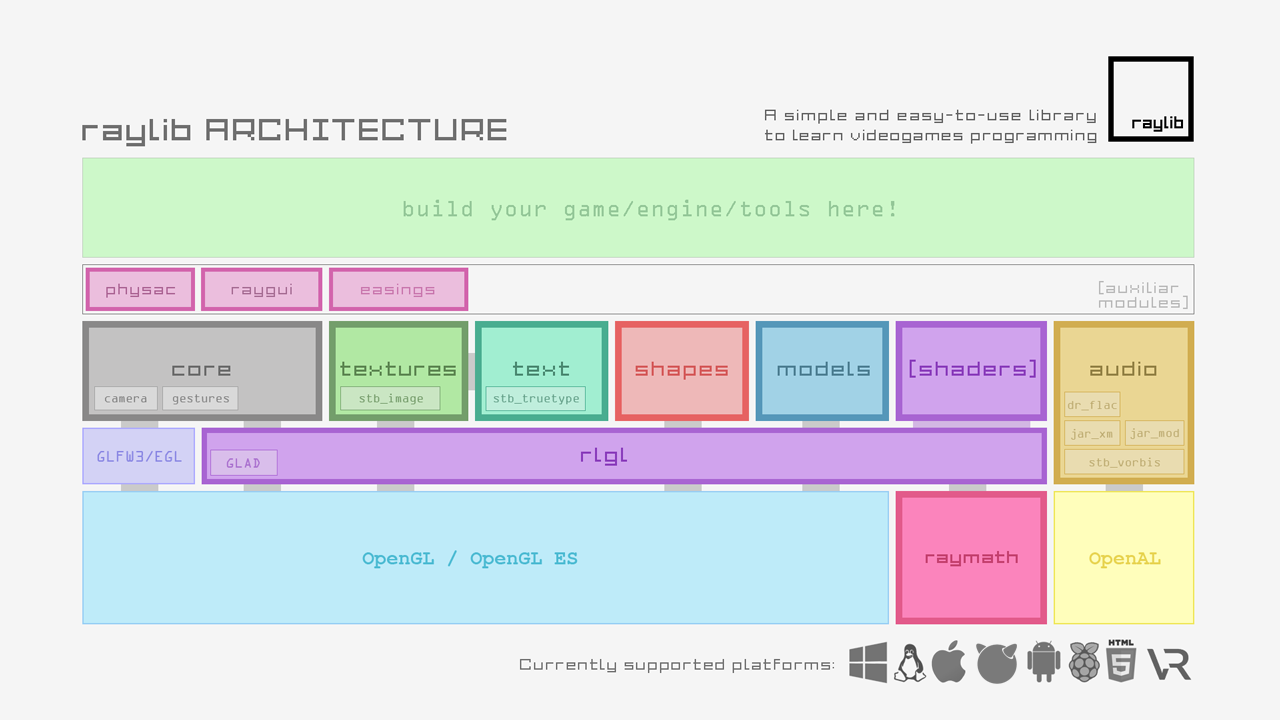
\includegraphics[width=12cm]{raylib_architecture}
	\caption{Arhitektura Raylib knjižnice. Vir \cite{raylib}}
	\label{slika:raylib}
\end{figure}

Sledijo ogrodja, ki sodijo v kategorijo visokonivojskih knjižnic in ogrodij. To so ogrodja, ki so zgrajena z namenom izdelave računalniških iger in tako ponujajo vso funkcionalnost, ki bi jo rabili. Imajo svoj način uporabe, vendar s tem znižajo potrebno delo, da uresničimo svoj cilj.

LibGDX je ogrodje za programski jezik Java. Je odprtokodno in podpira vse namizne platforme, kot tudi Android, iOS ter izvajanje v brskalnikih. Ima zelo močen pogon za izrisovanje 2D in 3D grafike, obenem pa ponuja dostop do nizkonivojskih funkcij če jih rabimo. Izrisovanje različnih objektov se zapakira skupaj, kar doprinese k hitrosti ogrodja. Podpira več vrst glasbenih in slikovnih formatov, delo z vhodnimi napravami ter gestami, ima obsežno funkcionalnost za matematične operacije, podpira 2D in 3D fizikalni pogon, mrežno komunikacijo, razna dodatna orodja in še veliko več. Skoraj vsa funkcionalnost, da izdelamo igro od začetka do konca, je v tem ogrodju. Ponuja scenski sistem za delo z našimi objekti v igri, kar nakazuje na specifičen način izdelovanje naše igre s pomočjo scen. Ni pa ta funkcionalnost obvezna \cite{libgdx}.

Monogame je ogrodje za programski jezik C\#. Ogrodje je nastalo kot nadomestek Microsoft-ega XNA ogrodja, ko je Microsoft prekinil podporo za XNA ter je kompatibilen z kodo, ki je bila spisana za obstoječo knjižnico. Dandanes se je Monogame skupaj z Mono ogrodjem razvil v kompletno rešitev za izdelavo računalniških iger. Podpira podoben nabor funkcionalnosti kot LibGDX z izjemo manjkajočega fizikalnega pogona. Tega lahko vključimo na primer z uporabo Box2D ipd. Monogame je odprtokoden in na voljo za vse večje platforme \cite{monogame}.

Cocos2D je zbirka različnih ogrodij za razvoj iger. Začetek razvoja je bilo ogrodje za programski jezik Python, nakar pa se je projekt odcepil v več ogrodij. Dandanes so v Cocos2D družini sledeča ogrodja: Cocos2D (originalno ogrodje za Python), Cocos2D-Swift (za programski jezik Swift in iOS platformo), Cocos2D-XNA (podobno kot projekt Monogame, je ta različica izdelana kot nadgradnja XNA ogrodja, danes pa deluje na Monogame), Cocos2D-JS (za programski jezik JavaScript ter razvoj računalniških iger za spletni brskalnik) in Cocos2D-X (največje ogrodje v tej družini, za programski jezik C++). Najbolj popularna veja ogrodja je Cocos2D-x, ki je tudi najbolj vzdrževana. Je odprtokodna in deluje na vseh večjih platformah. Ima zelo podoben nabor funkcionalnosti kot LibGDX in Monogame, ter vključuje tudi fizikalni pogon Box2D in Chimpmunk. Razvijalci Coco2D družine pa tudi ponujajo Cocos Studio, ki deluje kot namenski pogon za razvoj iger in bazira na Cocos2D-X ogrodju. Vsa ogrodja iz te družine bazirajo na delu s Sprite-i. Vsa logika se vrti okoli teh objektov, za to se moramo temu prilagoditi za produktivno delo v tem ogrodju \cite{cocos2d}\cite{cocos2dx}.

\subsection{Namenski pogoni}
Namenski pogoni so višek današnje tehnologije za razvoj računalniških iger. Na trgu obstaja več različnih pogonov, vendar daleč pred vsemi vodita razvoj Unity od Unity Technologies in Unreal Engine od podjetja Epic. Oba nudita svoj urejevalnik, v katerem grafično izdelujemo računalniško igro in tako pohitrimo razvoj, na voljo pa nam je vsa funkcionalnost, ki bi jo kdaj potrebovali. Vsak ima tudi svojo trgovino, v kateri lahko kupimo gradnike za igro ter dodatne funkcionalne razširitve za potrebe razvoja. Sta nekako zaprt ekosistem, v katerem razvijamo vse.

Unity je prvič izšel leta 2005. Pogon je zgrajen v programskem jeziku C++, razvijalcem pa ponuja vmesnik za namensko programiranje v C\#. Ponuja vso funkcionalnost, ki smo jo našteli v drugih knjižnicah in ogrodjih doslej, ter še veliko več. Pogon uporabljajo profesionalni studii po vsem svetu za razvoj iger in je najbolj priljubljen za individualne razvijalce med namenskimi pogoni. Glavne prednosti pred drugimi pogoni je preprosta uporaba, nizka stopnja potrebnega znanja, ogromen nabor dokumentacije in vodičev za izdelavo iger, hitro iskanje odgovorov (zaradi popularnosti hitro najdemo rešitev na našo težavo) ter velik nabor dodatne funkcionalnosti preko Unity trgovine kar iz orodja za razvijanje. Med funkcionalnostmi za razvoj ponuja tudi enostavno vgradnjo sistema za nakupovanje v naši igri ter oglase. Ponujajo tudi oglaševanje naše aplikacije skozi vse druge igre, ki uporabljajo Unity reklame in tako hitro dosežemo nove igralce. Za razvoj iger za več igralcev preko spleta imajo strežnike in integracijo kar preko Unity Editor-ja.

V preteklosti je bila določena funkcionalnost nedostopna zastonjskim uporabnikom, dandanes pa ni več omejitev. Edina omejitev pri zastonjski verziji je, da moramo obvezno pri zagonu naše igre prikazati Unity logotip, ter da so namenski strežniki za našo igro omejeni na 20 igralcev naenkrat. Zastonjska verzija nam je na voljo, če naše podjetje na leto zasluži manj kot sto tisoč dolarjev. Za prihodke od sto tisoč do dvesto tisoč potrebujemo Unity Plus licenco za 35 dolarjev mesečno, za večje prihodke pa potrebujemo Unity Pro licenco, ki stane 125 dolarjev mesečno. Plačljive licence dovolijo, da ne prikažemo Unity logotipa na začetku igre, več igralcev istočasno na njihovem strežniku, dodatno analizo za izdano igro, direktno podporo od Unity razvijalcev, 20\% popust na vse izdelke iz Unity trgovine in še več. Unity Technologies ponujajo tudi alternativo sistema za verzioniranje, ki nam omogoča lažjo sinhronizacijo med drugimi sodelavci in je vgrajen v Unity Editor \cite{unityFeatures}.

Unreal Engine ima daljšo zgodovino kot Unity, prvotna verzija pogona je izšla leta 1998. Prva in druga verzija nista bile na voljo za prosto uporabo, tretja verzija pa je pripeljala SDK za širšo uporabo. Četrta verzija pogona leta 2014 je zaznamovala začetek dostopnega in odprtokodnega namenskega pogona, ki ga je lahko uporabljal vsak. Pogon je razvit v jeziku C++ in v njem ponuja razvijalcem namenski programski vmesnik. Funkcionalnost je podobna Unity Engine-u vendar je večji poudarek na tehnološkem napredku in naprednih grafičnih izrisovanjih. Pogon je bolj priljubljen pri večjih profesionalnih studiih, ki hočejo izrabiti napredno funkcionalnost pogona. Glavne prednosti pred drugimi pogoni je prosto dostopna izvorna koda, večji in bolj tehnološko dovršen nabor funkcionalnosti, možnost vizualnega programiranja ter bolj dodelano in performantno jedro pogona. Licenciranje je drugačno od Unity-ja, uporaba je zastonjska brez omejitev, ko pa igro izdamo pa moramo podjetju Epic plačati 5\% vseh prihodkov igre \cite{unrealEngine}. 

Odločiti se med pogonoma je odvisno od naših potreb za projekt. Unity licenciranje in lažja dostopnost je prednost pri manjših projektih, kjer ne potrebujemo najnovejših funkcionalnosti za razvoj. Pri profesionalnih projektih začneta izstopati dve največji pomanjkljivosti Unity pogona. Prva je specifične manjkajoče funkcionalnosti, ki jih moramo nato za dodaten denar kupiti na Unity trgovini, ki so mogoče že privzeto vključene v Unreal Engine (Unreal Engine je bolj celovit paket pogona, kjer nam ni potrebno dodatnih funkcionalnosti doplačevati, kar je velika prednost). Druga pomanjkljivost Unity pogona pa je slabša grafična podoba, kot jo doseže Unreal Engine. Unity Technologies si trenutno zadaja cilj, da ti dve pomanjkljivosti odpravi, vendar je trenutno za bolj komplekse projekte priporočljiv Unreal Engine. Po drugi strani pa je prednost Unity-ja pred Unreal Engine boljša mobilna podpora in nižja potrebna strojna zmogljivost za igranje igre. Nižja potrebna računalniška moč je preferirana pri manjših ali individualnih projektih. Kakorkoli že, moramo za vsak projekt individualno oceniti, kaj potrebujemo in kateri pogon boljše ustreza našim potrebam.

\chapter{Razvoj računalniške igre}\thispagestyle{fancy}
\label{chapter:razvojIger}
\section{Uporabljena orodja}
V sklopu magistrskega dela smo se odločili, da izdelamo računalniško igro v treh različnih različnih orodjih za razvoj iger:
\begin{itemize}
	\item Knjižnica RayLib v programskem jeziku C++. Kot omenjeno je RayLib prehodna knjižnica med nizkonivojskimi in visokonivojskimi knjižnicami. Ima vso glavno funkcionalnost potrebno za razvoj vendar ji manjka olajševalna funkcionalnost, ki smo jo morali sami razvit. Tako je najbolj primerna za razvoj igre z nizkonivojskega zornega kota.
	\item Ogrodje LibGDX v programskem jeziku Java. Je eno izmen najbolj funkcionalno polnih ogrodij, ki še ni samo za sebe namenski pogon s svojim načinom dela. Zato je odlično za prikaza razvoja, kjer se ne podrejamo načinu dela z pogonom.
	\item Namenski pogon Unity. Najbolj popularni namenski pogon za razvoj iger je skoraj obvezno potrebno vključiti v primerjavo. Nudi ogromno funkcionalnost, nizko vstopno težavnost in preprostost za uporabo. Z Unity smo lahko prikazali enostavnost razvoja iger.
\end{itemize}

Poleg omenjenih zgornjih orodij smo še potrebovali orodja za izdelavo grafičnih in zvočnih gradnikov. Za izdelavo 2D gradnikov smo uporabili vektorsko orodje Inkscape ter izvozili slike v rastrski format. Za izdelavo 3D modelov smo uporabili Blender, saj kot omenjeno nudi vso potrebno funkcionalnost. Za izdelavo zvočnih efektov smo se poslužili orodja Bfxr ter zvoke pretvorili v ustrezni format z orodjem Audacity.

Med samim razvojem smo si razgradili delo na platformi Trello, ves napredek pa smo verzionirali s sistemom Git ter naš repozitorij hranili na platformi GitHub. Vsa vsebina izdelana za potrebe magistrskega dela (koda, gradniki, projekti in magistrsko delo v Latex formatu) je na voljo na sledeči povezavi: \url{https://github.com/cimpresovec/Masters}. Vsebina uporablja MIT licenco kar pomeni, da je prosto dostopna za uporabo brez restrikcij.

\section{Končni produkt}
Računalniška igra, ki smo jo izdelali v sklopu magistrskega dela je klon igre Breakout. Originalna igra je izšla leta 1976 za Atari, vendar je do danes izšlo na desetine variacij igre. V igri igralec kontrolira lopar, s katerim odbija žogo v omejenem prostoru. Lopar je omejen na spodnji del zaslona in se lahko premika samo horizontalno. Z odbijanjem žoge poskuša igralec uničiti vse ovire v stopnji, od katerih se žoga odbija ko jih uničuje. Cilj je čimbolj spretno odbijati žogo, nabrati čim več pik ter napredovati skozi stopnje z uničenjem vseh ovir. Če se žoga igralcu izmuzne, potem izgubi eno življenje ter lahko poskusi znova. Odbijanje žoge od loparja je prilagojeno, da ima igralec visoko stopnjo nadzora v katero smer se bo žoga odbila.

Vse verzije igre (C++, Java in Unity) so zaključene celote in vsebujejo naslednje glavne funkcionalnosti:
\begin{itemize}
\item Naslovni zaslon, kjer prikažemo naš logotip igre. Pri namenskem pogonu Unity smo morali še prikazati Unity logotip, saj smo uporabljali zastonjsko verzijo orodja. Zaslon lahko vidimo na sliki \ref{slika:naslovniZaslon}.
\begin{figure}[h]
	\centering
	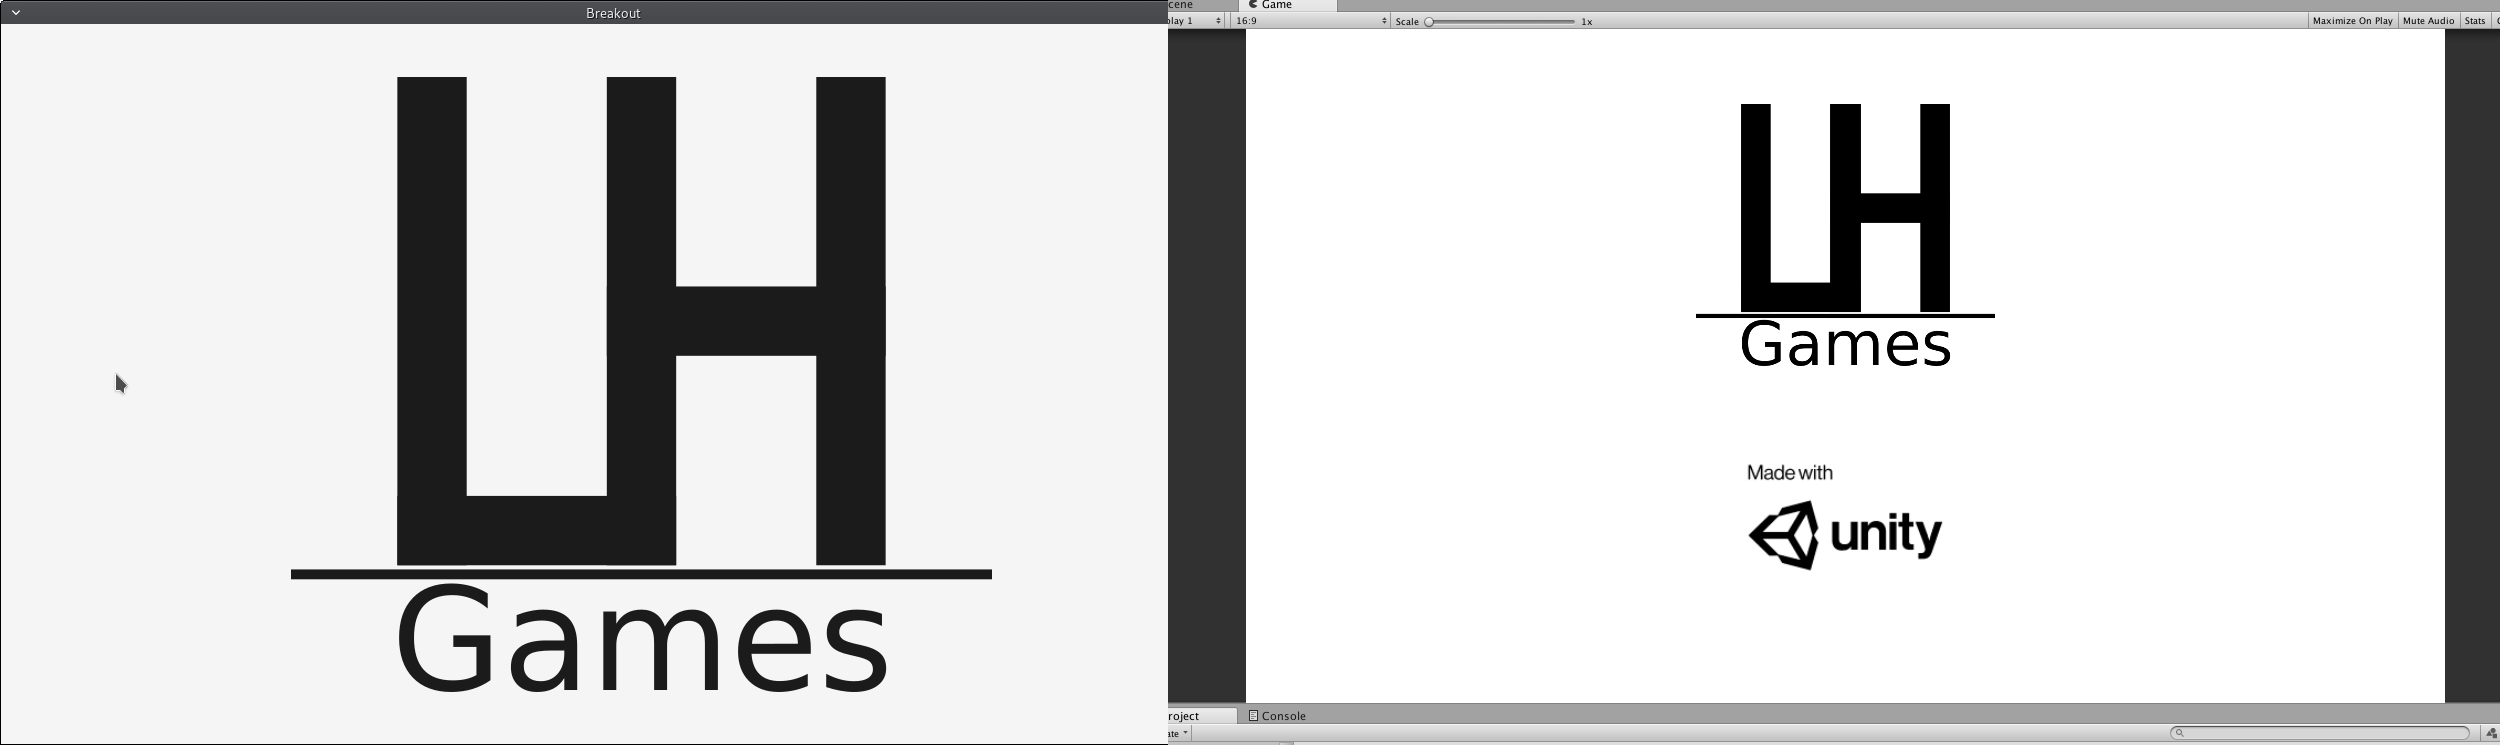
\includegraphics[width=14cm]{titleScreen}
	\caption{Naslovni zaslon. Levo v RayLib in LibGDX, desno v Unity.}
	\label{slika:naslovniZaslon}
\end{figure}
\item Glavni meni igre viden na sliki \ref{slika:mainMenu}. V glavnem meniju prikažemo naslov igre in nekaj dodatnih slik za popestritev zaslona. Uporabnik ima nato na voljo izbrati začetek igre, ali zapustiti aplikacijo.
\begin{figure}[h]
	\centering
	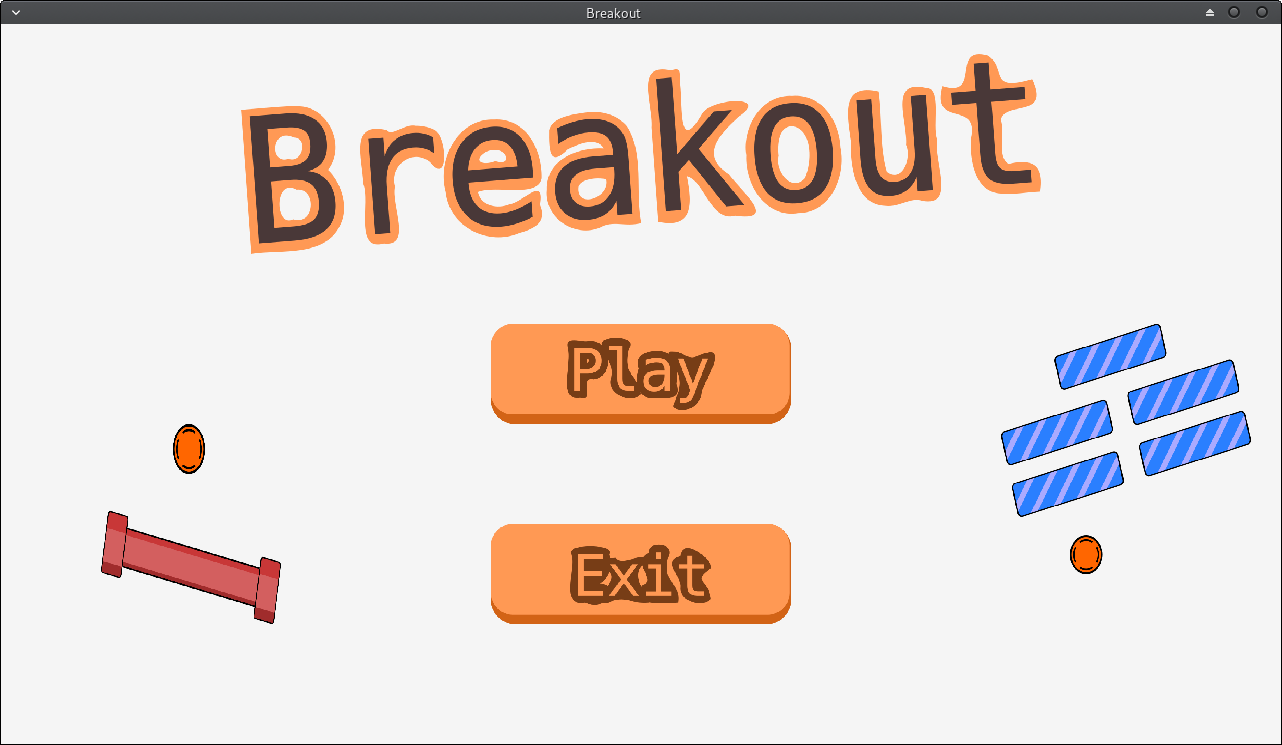
\includegraphics[width=14cm]{mainMenu}
	\caption{Glavni meni igre}
	\label{slika:mainMenu}
\end{figure}
\item Igralni del igre, ki je implementiran po zgornjem opisu. Z RayLib in LibGDX smo igro implementirali v 2D pogledu, kjer smo uporabili brezbarvne grafične gradnike, ki smo jih nato lahko individualno barvali med igranjem. V Unity pogonu smo igro implementirali v 3D pogledu z modeli, ki smo jih sami izdelali. Oba pogleda lahko vidimo na slikah \ref{slika:2dGame} in \ref{slika:3dGame}.
\begin{figure}[h]
	\centering
	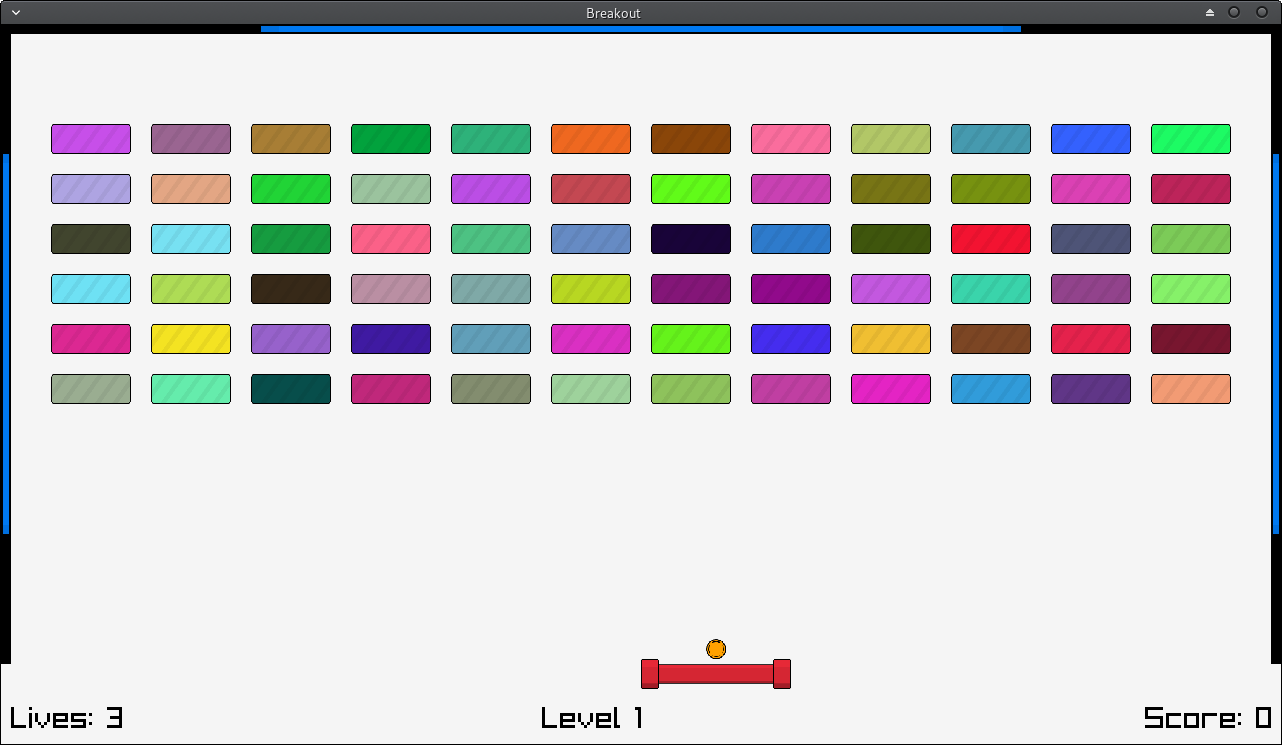
\includegraphics[width=14cm]{2dGame}
	\caption{2D variacija igre.}
	\label{slika:2dGame}
\end{figure}
\begin{figure}[h]
	\centering
	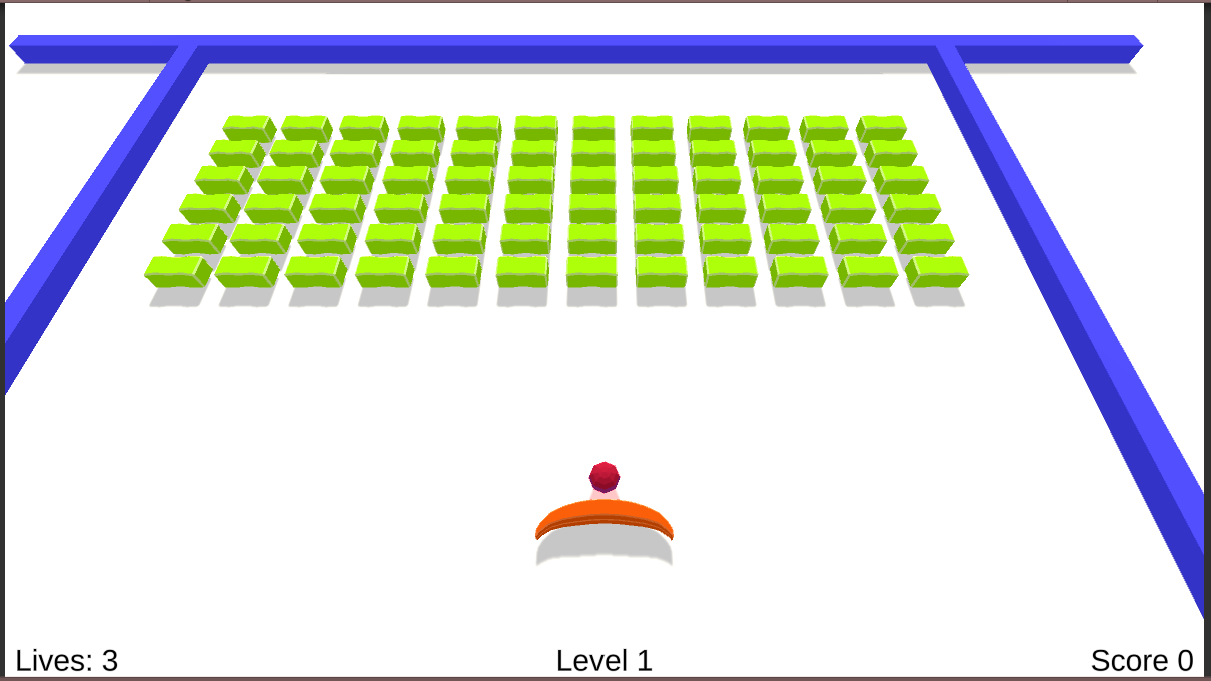
\includegraphics[width=14cm]{3dGame}
	\caption{3D variacija igre.}
	\label{slika:3dGame}
\end{figure}
\item Premikanje neodvisno od hitrosti izvajanja. Naše igre se obnašajo enako, neodvisno od zmogljivosti računalnika, na katerem se izvajajo.
\item Prehode med scenami z uporabo končnih avtomatov.
\item Upravljanje z grafičnimi in zvočnimi gradniki z direktorjem gradnikov.
\item Prilaganje izbrani resoluciji. Neodvisno od uporabnikovega zaslona, se naše igre prilagodijo brez rezanja prikazane vsebine.
\end{itemize}

Preostale funkcionalnosti kot so na primer teksturni atlas, fizikalni pogoni, ipd. smo implementirali samo v izbranih verzijah igre, saj niso tako korenito pomembne za razvoj. Vse uporabljene prakse in metode pa smo opisali v sledečih poglavjih magistrskega dela.

\section{Metode in prakse pri izdelavi grafičnih gradnikov}
\subsection{Barvno neodvisni slikovni gradniki}
Izdelavo 2D gradnikov si lahko olajšamo z omejitvijo barv, tako da uporabljamo samo sivine. Take slike so potem neodvisne od barve in jim lahko programsko izberemo barvo med igro. S tem si prihranimo čas, če se določeni objekti med samo razlikujejo samo po barvah (npr. preprosti nasprotniki, ovire v igri, ipd.). Spremembo barve v igri pa dosežemo z metodami za niansiranje.

V naši igri so vsi gradniki v 2D pogledu igre izdelani z to metodo. V sliki \ref{slika:grayscaleSprites} vidimo izdelane gradnike (od spodaj: lopar, ovira, žoga in desno zid) in v sliki \ref{slika:2dGame} vidimo končno uporabo v igri. Ovire v igri tvorijo lepo barvno paleto v resnici pa je uporabljen samo en grafični gradnik. Sprememba barve loparju in žogi je tudi trivialna, saj ni potrebno gradnika znova barvati v izbranem orodju. 

\begin{figure}[h]
	\centering
	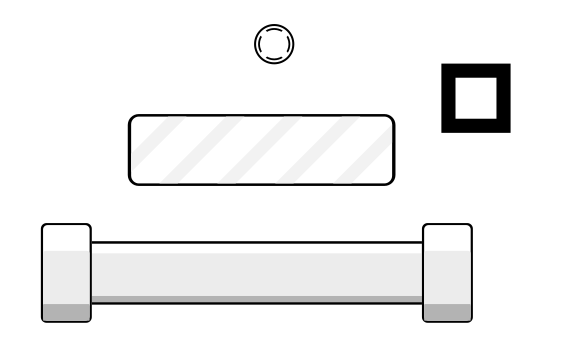
\includegraphics[width=8cm]{grayscaleSprites}
	\caption{2D sivinski gradniki}
	\label{slika:grayscaleSprites}
\end{figure}

Vsako orodje ponuja metode za niansiranje slik. Velikokrat izbrano barvo podamo kar v izrisovalno metodo. V RayLib nam metoda \textit{DrawTexturePro} ponudi šesti parameter, kamor vnesemo izbrano barvo. Primer lahko vidimo v izseku kode \ref{code:assetManager}. Če bi uporabljali barvno sliko, potem podamo v metodo belo barvo in s tem ne vplivamo na barvno nianso našega gradnika. V LibGDX niansiranje kontroliramo izven izrisovanje individualne slike. Razred \textit{SpriteBatch}, ki ga uporabljamo za izrisovanje ponuja metodo \textit{setColor(color)}, s katero izberemo nianso za vse nadaljnje izrise. Poskrbeti moramo le, da po uporabi spet nianso postavimo na belo in s tem ne pokvarimo preostalega izrisovanja.

Unity nam ponuja dva načina za niansiranje barv izrisovanja. Neodvisno ali izrisujemo 2D ali 3D gradnike potrebujemo material, ki določa lastnosti izrisovanja. Ena izmed lastnosti je niansa barve. Težava pri tej metodi je, da hočemo zaradi optimizacije uporabljati čimmanj različnih materialov, ki pa so potrebni, da individualno nastavljamo nianse. Tukaj se moramo odločiti, ali je bolj pomembno hitrost izrisovanja ali niansiranje sivinskih gradnikov. Malo število nians oz. materialov ne predstavlja velikega napora za Unity vendar se moramo zavedati mogočih posledic pri množični uporabi. Drugi način niansiranja je možen samo za 2D gradnike in je neodvisen od materialov. \textit{Sprite Rendered} komponenta, ki se uporablja za izrisovanje 2D gradnikov ponuja lastnost nianse slike, ki jo lahko uporabimo za naše namene. To lastnost lahko uporabljamo brez vpliva na zmogljivost vendar smo omejeni samo na 2D slike.

\subsection{Teksturiranje modelov z barvnimi paletami}
Teksturiranje modelov je obsežen proces, ki zahteva več korakov. Najprej je potrebno površino modela mapirat na 2D sliko brez vidnih deformacij nato pa na to sliko narisati želeno teksturo. S tem postopkom dobimo za vsak model svojo teksturo, ki jo uporabimo pri izrisovanju. Pri kompleksnih modelih je tak postopek zaželen, ko pa izdelujemo preprostejše modele (angleško low poly) hočemo ploskve modela preprosto obarvati z izbrano barvo. Takrat je prej omenjen postopek zamuden in potraten, obenem pa zaradi individualnih tekstur za vsak model izgubimo na zmogljivosti izrisovanja. Zato lahko pri preprostih modelih uporabimo metodo teksturiranja z barvnimi paletami.

Metoda za teksturo uporablja barvno paleto z naborom barv za vse naše modele. Tako lahko uporabimo samo eno teksturo za vse naše modele. Mapiranje modelov pri tej metodi je zelo preprosto, saj moramo individualne poligone modela mapirat v območje izbrane barve v teksturi. Na sliki \ref{slika:texturePalette} vidimo, da ni potrebno točno mapirati poligon, saj nam večji del teksture predstavlja izbrano barvo. 

\begin{figure}[h]
	\centering
	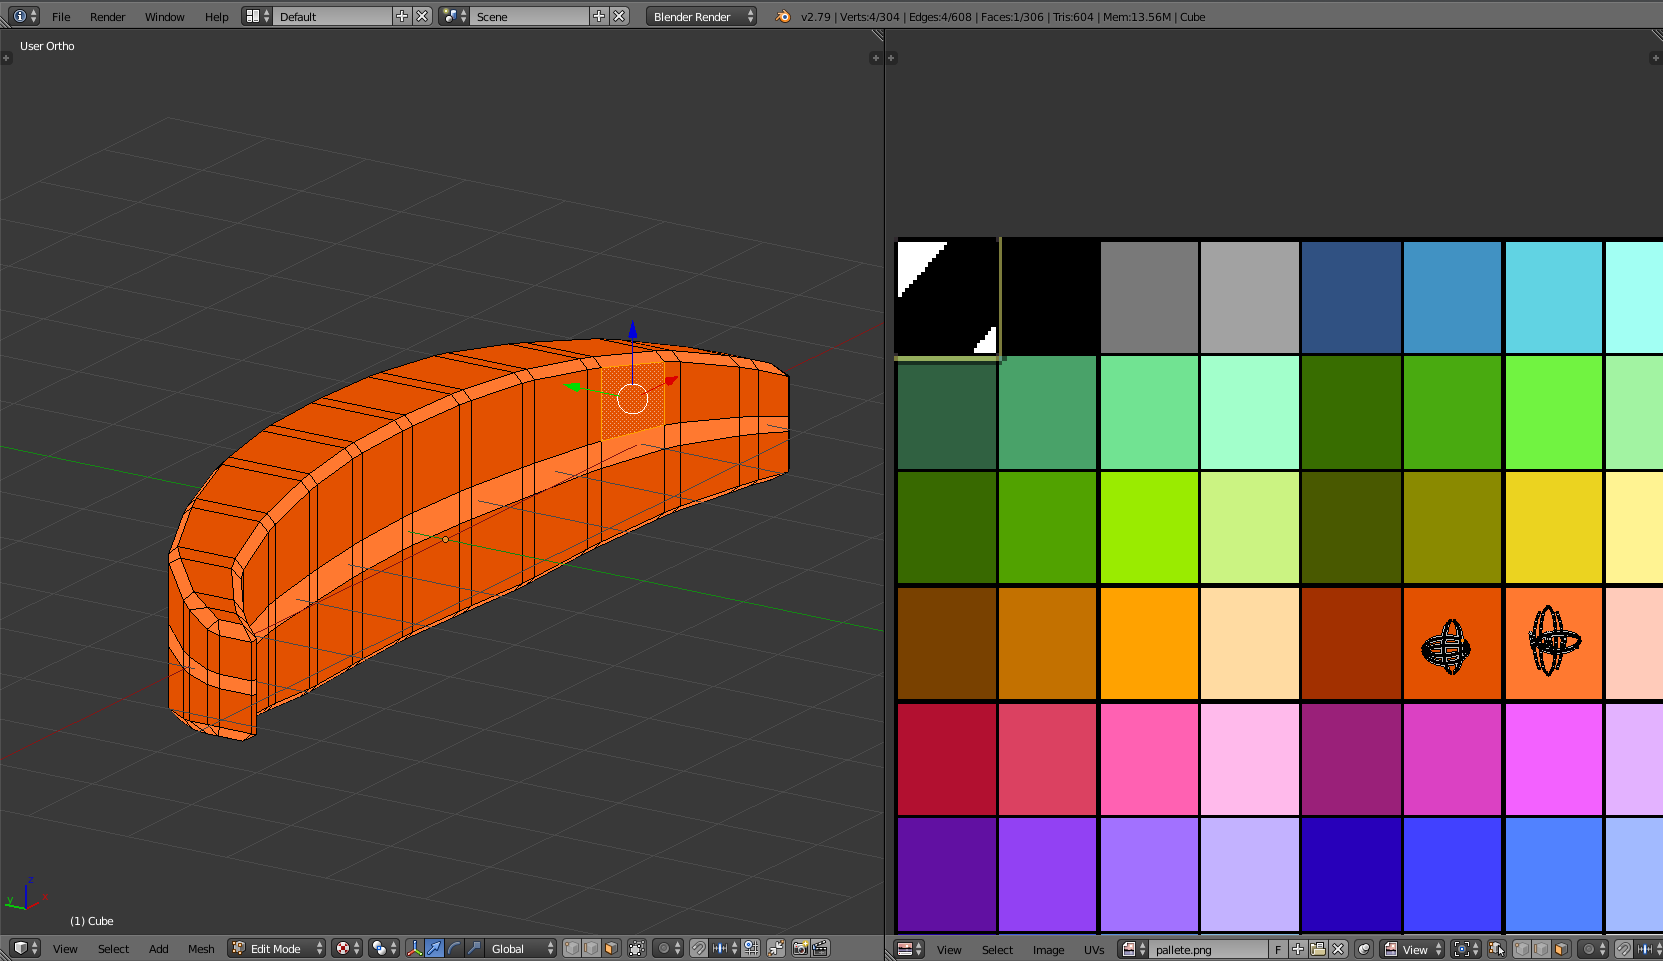
\includegraphics[width=14cm]{texturePalette}
	\caption{UV mapiranje preprostih modelov}
	\label{slika:texturePalette}
\end{figure}

S to metodo smo izdelali vse modele za našo igro. V pogonu Unity smo rabili samo en material za izrisovanje vseh modelov, zato je ta metoda tudi zelo performančna. Obenem metoda nudi dve veliki prednosti za spreminjanje barv med igro. Ker uporabljamo sliko barvne palete lahko to enostavno zamenjamo z drugo in tako preprosto zamenjamo barve na modelu ali celo na celotni sceni, če vsi modeli uporabljajo isto paleto. Tako lahko z enostavno menjavo dodamo večjo raznolikost našim stopnjam. Druga prednost te metode pa je lažje individualno menjavanje barv na modelu. Pri standardnem mapiranju, se skoraj nikoli programsko ne spreminjajo UV lokacije ogljišč, saj je mapiranje specifično za ta model. S to metodo je mogoče zaznati ogljišča, ki se nahajajo na izbrani barvi v teksturi in jih premestiti na drugo barvo. Tako lahko izbranemu objektu spremenimo izbrane barve. Je pa to menjavanje omejeno na vse poligone enake barve v modelu saj ni mogoče spremeniti barve samo enemu poligonu.

\subsection{Izvoz modelov za Unity}
Tips n tricks tukaj.

\section{Osnovne metode in prakse pri tehnični implementaciji}
Ne glede na izbiro orodij za tehnično implementacijo računalniške igre, so določene metode in prakse skupne vsem. Tudi če orodje poskrbi za določene prakse je dobro, da se jih zavedamo in tako boljše razumemo delovanje naših orodij in lahko bolj učinkovito implementiramo našo igro.

\subsection{Glavna zanka igre}
Glavna zanka igre skupaj z neodvisnim gibanjem od hitrosti izvajanja sta dva koncepta, ki sta specifična za igre v izdelavi programske opreme. Nekatera programska oprema se izvede in nato prikaže svoje rezultate brez kakršnihkoli vhodov, druga konstantno čaka na vhod ali dogodek od uporabnika, da proži akcije. Računalniške igre pa so konstantno v gibanju, tudi ko ne dobivajo vhoda od igralca. Če se igralec ustavi, se svet okoli njega v igri ne ustavi. Implementacija tega koncepta se imenuje glavna zanka igre. Psevdokodo preproste glavne zanke vidimo v izseku \ref{code:glavnaZanka}.

\begin{lstlisting}[label=code:glavnaZanka, language=C++, caption=Glavna zanka igre]
while(!shouldCloseGame)
{
	handleInput();
	update();
	render();
}
\end{lstlisting}

Kot vidimo je glavna zanka sestavljena iz treh glavnih delov: pridobitev in procesiranje vhoda od igralca, simulacija sveta igre in izris stanja na zaslon. Taka zanka se neskončno izvaja, dokler se igralec ne odloči, da igro zapre. Zagotavlja, da konstantno preverjamo vhode od uporabnika, odzovemo svet igre glede na ta vhod in nato takoj damo povratne informacije igralcu preko izrisa na zaslon. Za merjenje hitrosti izvajanja glavne zanke večinoma uporabljamo mero sličic na sekundo (angleško \textit{frames per second}), ki nam pove kolikokrat na sekundo se posodobijo informacije na zaslonu preko izrisa.

\subsection{Gibanje neodvisno od hitrosti izvajanja}
Hitrost izvajanja glavne zanke igre je zelo odvisna od specifikacij, ki jih premore strojna oprema na kateri igro izvajamo. Obremenjenost opreme je tudi faktor, če poleg igre izvajamo še druge procese. Tehnologija osveževanja zaslonov lahko tudi umetno omejuje hitrost izrisovanja in posledično tudi hitrost izvajanja zanke. Dandanes igre ciljajo dve hitrosti, to sta 30 ali 60 sličic na sekundo. Odvisno od tehnične zahtevnosti igre in ciljne platforme, saj konzole niso tako zmogljive kot namenski igralski računalniki. Ciljno hitrost najlaže dosežemo z umetnim čakanjem za izrisom. 

Neodvisno od ciljne hitrosti, pa v igri prihaja do nihanj. Določene scene zahtevajo več računalniških virov in tako povečajo potrebno procesorsko moč. Takrat se hitrost izvajanja zanke upočasni. Pri osnovnem modelu glavne zanke oziroma z modelom z umetnim čakanjem bi to pomenili upočasnitev same igre. Svet bi se simuliral počasneje in igralcu bi se zazdelo, kot da vse poteka v počasnem posnetku. Da se temu izognemo uporabljamo metode, ki simulirajo igro z enako hitrostjo neodvisno od hitrosti izvajanja glavne zanke. Najbolj popularna metoda uporablja merjenje časa, ki je pretekel od prejšnje izvedbe glavne zanke. Primer psevdokode vidimo v izseku \ref{code:deltaTime}.

\begin{lstlisting}[label=code:deltaTime, language=C++, caption=Neodvisno gibanje]
float previousTime = getCurrentTimeInMs();
while(!shouldCloseGame)
{
	float currentTime = getCurrentTimeInMs();
	float deltaTime = (currentTime - previousTime) / 1000.0f;
	handleInput();
	update(deltaTime);
	render();
	previousTime = currentTime;
}

void update(float deltaTime)
{
	position.x += 200 * deltaTime; //Hitrost premikanja je 200 enot na sekundo
}
\end{lstlisting}
Kot vidimo si izračunamo delta čas med ponovitvami. Dobra praksa je delto pretvoriti v sekunde saj jo je potem lažje uporabljamo v računske namene. Delta čas podamo v metodo, kjer se izvaja simulacija in ga uporabimo pri operacijah, ki so odvisne od hitrosti izvajanja. Tako lahko dosežemo, da se premikamo z konstantno hitrostjo na sekundo, ne glede na hitrost izvajanja glavne zanke.

Razvojna orodja nam ponujajo različne načine upravljanja z glavno zanko in delta časom. Pri nizkonivojskem programiranju si moramo sami ustvariti glavno zanko in se odločiti, kako se bo prožilo zaporedje dogodkov. Knjižnica Raylib nam ponuja metodo \textit{GetFrameTime()}, ki nam vrtne delta čas v sekundah. Pri tako dostopni metodi moramo paziti, da delta čas pridobimo samo enkrat v eni ponovitvi zanke. Če bi čas pridobili na več mestih, bi ta lahko bil različen in bi se objekti v naši igri simulirali z različnimi hitrostmi. Zato je ustaljena praksa, da čas pridobimo enkrat in ga nato predamo v nadaljnje metode.

Ogrodje LibGDX ima točno definirano glavno zanko na katero ne moremo vplivati. Moramo implementirati vmesnik \textit{ApplicationListener}, ki nam ponuja samo eno vstopno točko v zanko, metodo \textit{render()}. Ime metode je zavajajoče, saj ni namenjena samo za izrisovanje. Uporabiti jo moremo kot telo glavne zanke in v njej implementirati simulacijo igre in izrisovanje. Procesiranje vhodov se v LibGDX dela z proženjem dogodkov, ki poteka neodvisno od metode \textit{render()}. Za pridobitev delta časa nam je podobno kot pri Raylib na voljo metoda \textit{Gdx.graphics.getDeltaTime()}.

Pogon Unity ima zelo kompleksno glavno zanko razdeljeno na več delov (simulacija fizikalnega pogona, proženje dogodkov, simulacija igre, izrisovanje scene, izrisovanje uporabniškega vmesnika, ipd.). Z našimi objekti se lahko vključimo v vsak posamezen korak glavne zanke. Unity poleg simulacije igre še izvaja simulacijo fizikalnega pogona, ki se lahko izvede večkrat v eni iteraciji glavne zanke. Metodi za delo s simulacijama sta \textit{FixedUpdate()} (simulacija fizikalnega pogona) in \textit{Update()} (preostala simulacija). Za pridobitev delta časa pa nam je na voljo metoda \textit{Time.deltaTime}.

%TODO MOGOCE OPISATI DETERMINISTIČEN KORAK ZA SIMULACIJOs
\subsection{Upravljanje stanj v igri}
Upravljanje stanj je mišljeno kot organizacija in prehajanje med stanji kot so začetni logotip, različni meniji igre (glavni meni, meni za izbiro stopenj, ipd.) in različnimi nivoji igre. Stanja so uporabna, saj lahko ločimo našo igro na individualne dele, ki se izvajajo neodvisno na druga stanja. Za stanja se uporablja tudi sinonim scena. Vsako ogrodje in namenski pogon ima svoj način dela s stanji, vendar so večinoma to preprosti končni avtomati, ki imajo definirane prehode med scenami in hranijo vsak svoje interne objekte. Ti interni objekti so potem gradniki uporabljeni v sceni igre. Med samo igro je to igralec in objekti v svetu, v meniju so gradniki grafičnega vmesnika, ki se odzivajo na dogodke, ipd.

Pri nizkonivojskih knjižnicah smo sami implementirali prehode med scenami. Za osnovo potrebujemo abstraktni razred, ki bo ogrodje za glavne metode scene (deli glavne zanke igre). Primer vidimo v izseku \ref{code:stanjeIgre}.

\begin{lstlisting}[label=code:stanjeIgre, language=C++, caption=Stanje igre]
enum GameStates {STATE_NULL, STATE_TITLE, STATE_LEVEL, STATE_EXIT};

class GameState {
	protected:
		GameStates currentGameState = GameStates::STATE_NULL;
		GameStates nextGameState = GameStates::STATE_NULL;
	public:
		virtual ~GameState();
		virtual void handleEvents() = 0;
		virtual void handleLogic(const float deltaTime) = 0;
		virtual void handleRendering() = 0;
		GameStates getNextState() const;
		void changeGameState(const GameStates state);
};
\end{lstlisting}

Pri taki zasnovi smo nato preprosti dedovali od razreda \textit{GameState} in implementirali individualna obnašanja scen. Vsaka scena poskrbi za konstrukcijo in destrukcijo svojih objektov, med sabo pa si delijo skupne vire (kot recimo grafični in glasbeni gradniki). V glavni metodi naše aplikacije smo z uporabo polimorfizma ustvarili instanco enega stanja igre ter preprosto klicali namenske metode glavne zanke (izsek \ref{code:uporabaStanja}). V metodo za simulacijo igre smo podali delta čas, ki smo ga omenili v prejšnjem poglavju. Tako smo poskrbeli, da je delta čas enak skozi celotno simulacijo v enem koraku.

\begin{lstlisting}[label=code:uporabaStanja, language=C++, caption=Uporaba stanja igre]
std::unique_ptr<GameState> currentState = std::make_unique<LevelState>();

while (currentState->getNextState() != STATE_EXIT) {
	currentState->handleEvents();
	currentState->handleLogic(GetFrameTime());
	currentState->handleRendering();
	if (currentState->getNextState() != STATE_NULL) switchGameState(currentState);
} //...
\end{lstlisting}

Ogrodje LibGDX nam ponuja vmesnik \textit{Screen}, ki deluje podobno kot naš implementiran \textit{GameState} razred. Upravljanje z scenami smo morali implementirati sami, saj ogrodje nima implementiranega svojega načina. Pri tem smo upoštevali enake principe kot pri nizkonivojski knjižnici. LibGDX nam edino olajša prehode med scenami, saj razred \textit{Game} ponuja metodo \textit{setScreen}, ki enostavno uniči trenutno sceno in naloži novo. Mi smo samo implementirali transformacije, kdaj se katera scena naloži.

Unity ima svoj sistem upravljanja s scenami, vendar je v ozadju zelo podoben temu v LibGDX. V grafičnem urejevalniku smo ustvarili posamezne scene in jih shranili s končnico \textit{.unity}. Vse možne scene nato naštejemo v nastavitvah naše aplikacije, nakar nam Unity ponudi singleton \textit{SceneManager} za upravljanje prehodov. Dve glavni metodi za prehode med scenami sta \textit{LoadScene} in \textit{LoadSceneAsync}. Noter podamo ime scene, pogon jo naloži in nato zamenja obstoječo sceno. Razlika med metodama je edino, da prva blokira izvajanje med nalaganjem, druga pa naloži sceno v ozadju. Privzeto se celotna obstoječa scena zamenja z novo, ponuja pa Unity nalaganje scen ene v drugo. Tako lahko naložimo več različnih scen in jih družimo v želeno celoto. Ta princip je uporaben, če imamo del scene vedno enak (statičen, recimo igralčev lik), preostanek scene pa so možne različne variacije.

\subsection{Resolucija igre}
Zasloni, na katerih se bo naša igra prikazovala imajo različne resolucije in razmerja med horizontalno ter vertikalno dolžino. Te razlike lahko privedejo do nepričakovanih sprememb pri izrisovanju, če razlik nismo predvideli. Najhuje je, ko se del scene ne izriše, ker je resolucija igre ožja od pričakovane. Primer lahko vidimo na sliki \ref{slika:rezanje}. Z črno obrobo je prikazana resolucija zaslona oziroma okna igre, z temno rdečo pa prikazano sceno. Prvi primer prikazuje optimalno izrisovanje, primer 2 in 3 pa težave, ki nastanejo, če ne poskrbimo za različne resolucijo. Kot vidimo iz slike, določeni deli scene niso več videni na zaslonu.

\begin{figure}[h]
	\centering
	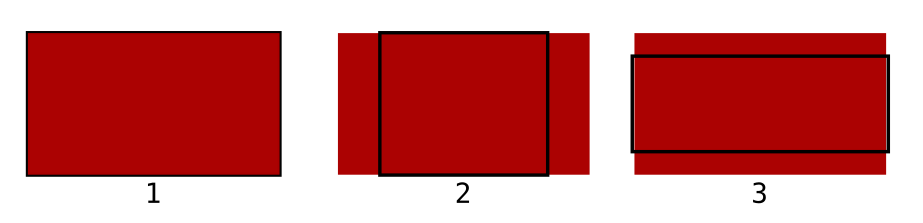
\includegraphics[width=12cm]{rezanjeResolucije}
	\caption{Primeri izgubljenega dela scene.}
	\label{slika:rezanje}
\end{figure}

Za reševanje teh težav nam orodja večinoma ponujajo delo s kamerami ali pogledi na sceno. Z njimi lahko krmilimo, kako se bo izrisovanje odzivalo na različne resolucije. Igro ko razvijamo večinoma zasnujemo z določeno resolucijo in razmerjem v mislih, nato pa poskrbimo za potrebna prilagajanja. Na voljo imamo več načinom: lahko se odločimo, da bomo ohranjali razmerje ali ne. Če originalnega razmerja ni potrebno ohranjati, potem lahko izrisovanje prilagodimo novi resoluciji in izris preprosto raztegnemo na uporabnikovem zaslonu. Pri tem lahko pride do popačenj, vendar vedno zapolnimo razpoložljivo resolucijo. Če hočemo ohranjati originalno razmerje, pa moramo skleniti določene kompromise. Ti kompromisi so črni oziroma prazni deli zaslona, saj če se uporabnikovo razmerje resolucij ne sklada z zasnovano potem ni mogoče popolnoma prilagoditi izrisovanja. Primera prilagajanja vidimo na sliki \ref{slika:prilagajanje}. V primeru 1 je uporabnikova resolucija ožja od zasnovane, zato smo izris prilagodili. Zaradi ohranjanja originalnega razmerja imamo na vrhu in dnu zaslona prazne dele. Primer 2 je ravno nasproten scenarij.

\begin{figure}[h]
	\centering
	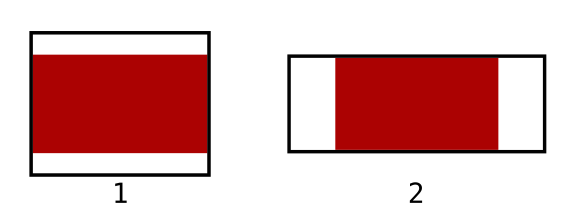
\includegraphics[width=10cm]{prilagajanje}
	\caption{Primeri prilagajanja izrisovanja.}
	\label{slika:prilagajanje}
\end{figure}

Knjižnica RayLib ponuja razred \textit{Camera2D} za upravljanje z resolucijami. Podpira samo prilagajanje s ohranjanjem razmerja, saj ni mogoče spreminjati horizontalne in vertikalne povečave neodvisno, le s skupnim faktorjem preko \textit{zoom} spremenljivke. Kameri še nato postavimo izvirno velikost in pozicijo ter jo nato uporabimo pred začetkom izrisovanja s metodo \textit{Begin2dMode()}. Ko zaključimo izrisovanje uporabimo metodo \textit{End2dMode()}. Ti metodi poskrbita, da se vso izrisovanje prilagodi parametrom kamere.

LibGDX ogrodje ponuja veliko bolj dovršen način upravljanja s resolucijami z uporabo razredov \textit{Camera} in \textit{Viewport}. Na voljo nam je več specializacij razreda \textit{Viewport}. \textit{StretchViewport} prilagaja resolucijo brez ohranjanja originalnega razmerja, \textit{FitViewport} ohranja razmerja, vendar pušča prazne predele. Obstaja še \textit{FillViewport}, ki podobno kot \textit{FitViewport} ohranja razmerje, vendar ne pušča praznih predelov ampak poveča izris izven zaslona, tako da določeni deli scene niso videni. Uporaba razredov je preprosta, saj jih le instanciramo z želeno originalno resolucijo nato pa podobno kot pri RayLib uporabimo metodo \textit{setProjectionMatrix} pred izrisovanjem.

Unity ponuja kamera objekte za prilagajanje resolucij. Igre v Unity so vedno 3D, tudi kadar uporabljamo 2D komponente, zato kamere delujejo za 3D svet. To pomeni, da ni mogoče na enostavni način prilagajati izrisovanje z ohranjanjem originalnega razmerja. Če hočemo ohranjevati razmerje, je potrebno v izrisovanje vključiti vmesni korak, to je izrisovanje na teksturo, katero nato prilagodimo in jo prikažemo na zaslonu. Če pa nočemo ohranjevati razmerja in prilagoditi originalni izris kakršnikoli resolucijo pa enostavno nastavimo aspekt komponento kameri na želeno originalno vrednost in Unity avtomatsko prilagodil izris.

\subsection{Upravljanje s grafičnimi in glasbenimi gradniki}
Singleton za assete v C++, libgdx. Kako upravlja resource unity.
Upravljanje s grafičnimi in glasbenimi gradniki je pomemben del razvoja igra. Ti gradniki predstavljajo po velikosti največji del naše igre, zato se moramo odločiti kako jih bomo uporabljali. Ker so ti gradniki veliki, jih nočemo nalagati med samim igranjem, saj potem lahko pride do nepotrebnih zastojev med igranjem. Nalaganje se večinoma dogaja na samem začetku pogona igre ali v vmesnih scenah, ki so specifično namenjeni za to. Nalaganja med igranjem se samo poslužujemo, če so naši gradniki preveliki (ko velikosti začnejo dosegati gigabajte), takrat obstajajo tehnike za sprotno nalaganje.

V naših igrah gradniki niso bili preveliki zato smo se odločili, da jih vse naložimo ob zagonu igre. Pogon Unity dela z gradniki drugače in jih naloži ko nalagamo sceno v kateri je gradnik uporabljen. Neodvisno od uporabljene strategije, pa je pomembno, da gradnike ločimo od drugih komponent v naši igri in jih naložimo samo enkrat. Če bi gradnik vezali na objekt v igri kot na primer strelivo, potem bi konstantno prihajalo do nalaganja in odlaganja grafičnega gradnika, ko bi igralec streljal, čez čas pa bi strelivo izginilo zaradi optimizacije. Takega delovanje si ne želimo saj hočemo, da je isti grafični gradnik uporabljen za vso strelivo. Za tako upravljanje uporabljamo princip direktorja gradnikov, kateri hrani vse potrebne gradnike in jih daje na voljo drugim objektom. Velikokrat se ti direktorji poslužujejo singleton principa, saj nočemo več instanc direktorja gradnikov.

V C++ smo si sami ustvarili direktorja, saj knjižnica Raylib ne ponuja take funkcionalnosti. Naš direktor je hranil mapo tekstur in zvokov, do katerih smo dostopali preko imen, ki smo jih priredili gradnikom. Direktor je bil singleton, ki je bil na voljo vsem objektom v igri. Nalaganje gradnikov pa smo izvršili pred začetkom glavne zanke igre. V izseku \ref{code:assetManager} vidimo primer uporabe. Prvi dve vrstici prikazujeta nalaganje gradnikov pod nekim imenom, tretja vrstica pa prikazuje kasnejšo uporabo pri izrisovanju. 

\begin{lstlisting}[label=code:assetManager, language=C++, caption=Uporaba direktorja gradnikov]
AssetManager::getInstance().loadTexture("pad", "../assets/pad.png");
AssetManager::getInstance().loadSound("blip", "../assets/blip.wav");
DrawTexturePro(AssetManager::getInstance().getTexture("wall"), AssetManager::getInstance().getRectangle("wall"), renderRectangle, Vector2{0, 0}, 0, BLUE);
\end{lstlisting}

Ogrodje LibGDX ponuja direktorja že v svoji funkcionalnosti pod imenom \textit{AssetManager}. Ponuja metodi \textit{load(path, type)} in \textit{get(path, type)}, ki upravljajo z gradniki. V LibGDX direktor privzeto ni singleton, zato ga tukaj nismo spremenili v singleton. Prvotno smo ga ustvarili v vhodni metodi v igro, in si instanco predajali med scenami in končno tudi samim objektom v metode, kje so potrebovali gradnike (npr. za izrisovanje). Druga pomembna razlika direktorja v LibGDX je, da gradnike nalaga asinhrono, pri čimer Raylib nalaga sinhrono. V LibGDX lahko z metodo \textit{finishLoading()} direktorja prisilimo, da dokonča nalaganje preden nadaljujemo z izvajanjem in se tako izognemo napakam zaradi nepopolnega nalaganja.

Pogon Unity kot že omenjeno dela drugače z gradniki. V ozadju naloži gradnike ko pride do nalaganje same scene. Gradniki so v urejevalniku direktno povezani z objekti v igri, vendar v ozadju Unity poskrbi, da so to dejansko isti gradniki in da ne pride do nepotrebnega nalaganja in odlaganja. Za naknadno nalaganje Unity ponuja dva mehanizma. Prvo je posebno imenovana mapa \textit{Resources}, kjer shranimo gradnike, ki jih bomo uporabljali za ta namen. Nato lahko med izvajanjem uporabljamo sinhrono metodo \textit{Resources.Load(name, type)} ali asinhrono metodo \textit{Resources.LoadAsync(...)}. Ko gradnikov več ne rabimo, jih lahko odložimo z metodo \textit{Destroy()} in \textit{Resources.UnloadUnusedAssets()}. Drugi način nalaganje gradnikov med izvajanjem so tako imenovani paketi sredstev (angleško asset bundle). To so skupki več gradnikov, ki jih lahko ustvarimo v urejevalniku in uporabniku dostavimo neodvisno od igre. Tako lahko izdelamo dodatke ali popravke za naši igro, brez da bi bilo potrebno ponovno prevesti našo igro. Te pakete nato med izvajanjem igre naložimo z metodama \textit{AssetBundle.LoadAsset(name)} in \textit{AssetBundle.Unload()}. 

\subsection{Teksturni atlasi}
Teksturni atlasi so najbolj pogosta optimizacija slikovnih grafičnih gradnikov. Ti gradniki se uporabljajo pri 2D igrah kot grafični liki pri 3D igrah pa kot teksture na modelih. Za izrisovanje na zaslon je najbolj performančno, če čim več izrisov združimo skupaj v enega. Združevanje pa ni možno, če izrisi rabijo različne slikovne grafične gradnike. Zato je potrebno, da te gradnike združimo v en večji grafični gradnik iz katerega potem preberemo le tisti del, ki ga potrebujemo. Ker pa ni potrebno menjati gradnika v ozadju lahko take izrise združimo v enega. Temu principu rečemo teksturni ali slikovni atlas.

Prvi korak za uporabo teksturnih atlasov je sama izdelava le-teh. Lahko se odločimo, da ročno iz več manjših slik ustvarimo eno večjo, vendar je to potratno saj obstaja veliko različnih orodij za ta namen. Orodja slike združijo na najbolj optimalni način, tako da ostane čim manj neizkoriščenega prostora za teksturnem atlasu. Prazen prostor po nepotrebnem troši spomin grafične kartice zato ga hočemo minimizirati. Ogrodje LibGDX ponuja svoje orodje za izdelavo atlasov pod imenom GDX Texture Packer GUI\footnote{https://github.com/crashinvaders/gdx-texture-packer-gui}. S tem preprostim grafičnim vmesnikom izberemo slike, ki jih hočemo zapakirati, nastavimo parametre obdelave in poženemo obdelavo. Z orodjem je možno kontrolirati kakovost končne slike, algoritem pakiranja, ipd. Orodje lahko vidimo levo na sliki \ref{slika:texturePacker}. Orodje nam poleg končne slike še izdela datoteko, ki hrani vse potrebne podatke za uporabo teksturnega atlasa.

\begin{figure}[h]
	\centering
	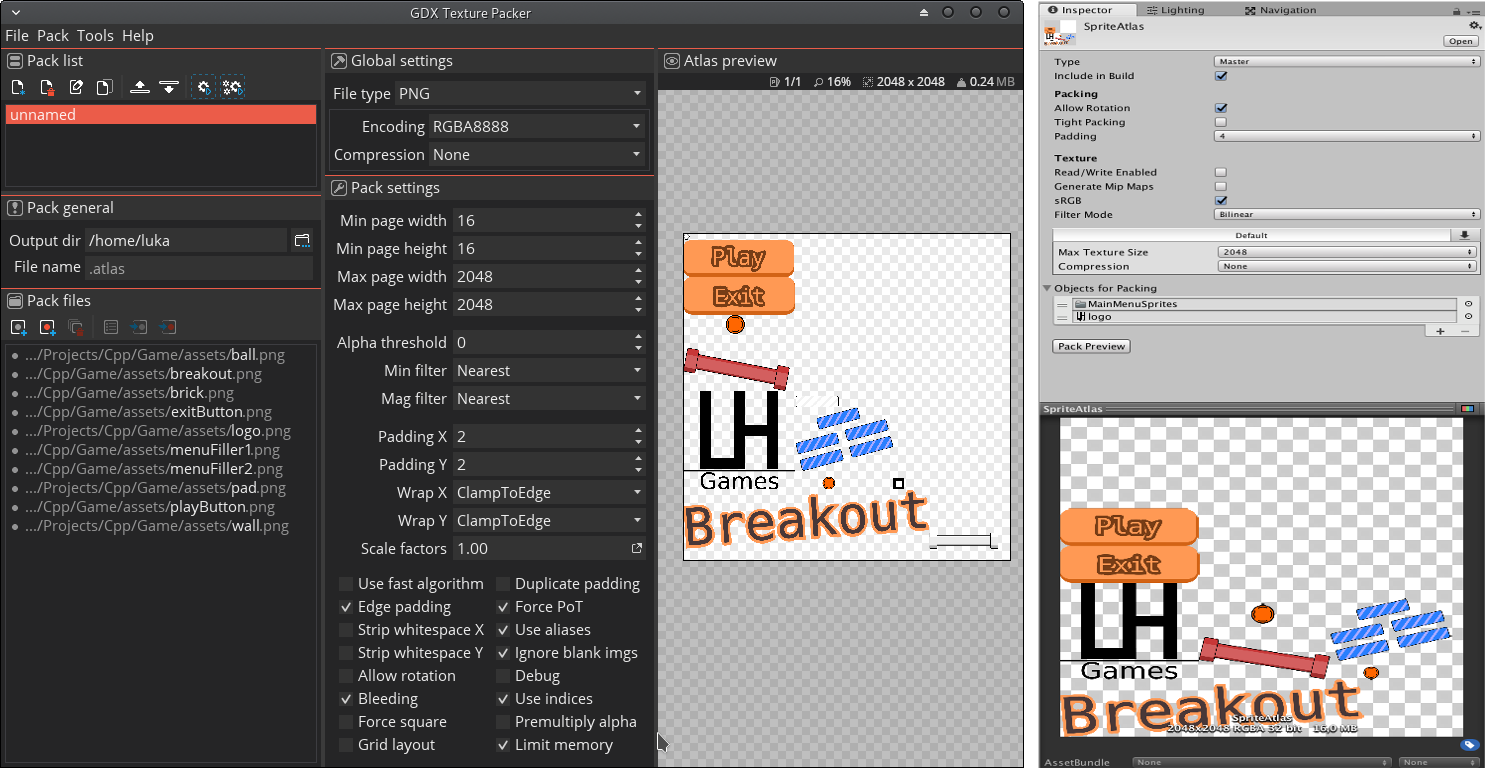
\includegraphics[width=15cm]{texturePacker}
	\caption{GDX Texture Packer GUI in Unity Sprite Packer}
	\label{slika:texturePacker}
\end{figure}

Unity urejevalnik omogoča še lažjo podporo teksturnim atlasom. Potrebno nam je samo omogočiti uporabo atlasov in nato specificirati, katere slike bodo uporabljene v atlasi. Unity potem avtomatsko poskrbi, da so izbrane slike uporabljene iz atlasov in tako uporabniku ni potrebno skrbeti za implementacijo. Kot vidno iz desnega dela slike \ref{slika:texturePacker}, nam Unity prikaže, kako bo izgledal končni teksturni atlas.

Uporaba teksturnih atlasov v Raylib in LibGDX zahteva dodatno delo za razliko od Unity pogona. Raylib nam ne ponuja nobene funkcionalnosti za podporo atlasov, tako da je potrebno implementirati uvoz ustvarjene datoteke z informacijami o atlasu. LibGDX pa ponuja potrebno funkcionalnost za delo z atlasom, ki so ustvarjeni z njihovim orodjem. Razred \textit{TextureAltas} nam omogoča branje ustvarjenih .atlas datotek nakar nam ponuja metode kot so \textit{findRegion(name)} in \textit{createSprite(name)}, da pridobimo ustrezne podatke za želeno izvorno sliko. Te informacije nato uporabimo pri izrisovanju podobno, kot da bi izrisovali posamezne slike. 

\section{Specifične metode in prakse pri tehnični implementaciji}
\subsection{Fizikalni pogoni}
Za realistično simulacijo fizikalnih objektov potrebujemo fizikalni pogon. Kot že omenjeno sta najbolj popularna pogona za 2D simulacijo Box2D in Chimpmunk. Za 3D simulacijo pa so med bolj znanimi Bullet, Physix in Havoc. Neodvisno od pogona pa pri vseh srečamo iste koncepte, prakse in gradnike, ki jih je potrebno razumeti za uporabo le-tega. Zato smo najbolj pomembne sklope pogonov opisali v našem delu:
\begin{itemize}
	\item \textbf{Simulacijski svet}.  Vsa simulacija se dogaja v tako imenovanem simulacijskem svetu. Ta je odgovoren za vsa telesa v simulaciji in nadzira dogajanje simulacije. Večinoma uporabljamo samo en simulacijski svet saj interakcije med svetovi niso podprete. Svet se ne simulira samostojno in brez naše interakcije obstoji na miru, zato obstajajo specifične metode s katerimi simulacijo poženemo naprej za določen čas. Klicanje teh metod vežemo na glavno zanko igre v simulacijski del zanke. S svetovi tudi krmilimo glavne parametre fizikalne simulacije kot so smer in moč gravitacije ter število iteracij pri reševanju trkov. Večje kot je število iteracij, bolj natančni in resnični so odzivi na trke.
	\item \textbf{Toga telesa (angleško rigid body)}. Toga telesa so osnova za vse objekte v fizikalnem svetu. Telesa ne predstavljajo oblike in velikosti objektov (to vlogo imajo konstrukcije) temveč lastnosti kot so: masa, hitrost  in smer gibanja, rotacijska inercija, rotacijska hitrost, lokacija in nagib. S pomočjo teh lastnosti in konstrukcije lahko nato razrešujemo trke med objekti.
	
	Vsi pogoni poznajo tri tipe togih teles: dinamično, statično in kinematično. Dinamična telesa predstavljajo vse objekte, kot jih poznamo v realnem svetu. Ti objekti se odzivajo na vse zunanje in notranje sile in se pri trkih realistično odzovejo. Dinamična telesa uporabljamo, ko hočemo simulirati realistično dogajanje v naši igri. Statična telesa ne obstajajo v realnem svetu saj so to telesa, ki se na sile in trke ne odzivajo. Neodvisno od moči trka se ta telesa ne bodo premaknila (druga telesa se vedno odbijejo od njih), obenem pa jih ni možno premakniti v kodi. Statična telesa uporabljamo za statične dele nivojov v igri (tla, zid, ipd.), ki nočemo da se premikajo vendar morejo vseeno obstajati kot ovira za dinamična telesa. Kinematična telesa so zelo podobna kot statična telesa, le da jih je možno v kodi premikati po svetu. Ta telesa uporablja za še vedno neodzivne dele nivojev, ki pa se morajo premikati po določenih smernicah (npr. premikajoča tla).
	\item \textbf{Konstrukcija (angleško fixture).} Konstrukcije so druga osnovna komponenta za fizikalno simulacijo. Predstavljajo obliko, velikost in materialne lastnosti objekta, priredimo pa jih na toga telesa. Odvisno od konstrukcije se telesu nato preračuna masa. Skupaj tvorijo predstavitev naših objektov v fizikalnem svetu. Lastnosti konstrukcije so gostota, trenje in moč odboja. Oblika konstrukcij je v veliko pogonih omejena na konveksna telesa, če pa hočemo simulirati konkavna telesa pa uporabimo dve ali več konveksnih konstrukcij, ki jih priredimo enemu togemu telesu.
	\item \textbf{Sile in impulzi}. Za realistično premikanje dinamičnih teles uporabljamo sile in impulze. Sile delujejo na telesa skozi čas, impulzi pa v trenutku prenesejo moč na telo. Oboje lahko uporabljamo za premikanje po prostoru ter za rotacijo teles. Ko uporabljamo sile in impulze vedno povemo moč in lokacijo sile ali impulza, saj nočemo vedno uporabiti sile v centru mase objekta.
	
	Telesa lahko premikamo po svetu tudi z direktnim nastavljanjem lokacije. To ni realistično premikanje s pomočjo sil zato lahko pride do nerealističnih odzivov drugih teles, če pride do trkov. Direktnemu premikanju se je zato najboljše izogniti in uporabljati sile in impulze. V realnem svetu se vse premika s pomočjo le-teh zato si lahko prihranimo neznane težave pri simulaciji z izogibanjem direktnega premikanja. Je pa ta metoda potrebna za posebne načine premikanja v igrah kot na primer teleportiranje. Podobno kot direktno nastavljanje lokacije ni priporočeno direktno nastavljati hitrosti gibanja, smeri gibanja in rotacijsko hitrost saj pride do enakih težav pri simulaciji.
	\item \textbf{Sklepi (angleško joint)}. Telesa lahko v svetu med samo povezujemo s sklepi. Ti predstavljajo zgibe, vrvi (elastične, toge), zvare, ipd. Z njimi lahko ustvarimo kompleksnejše objekte v naši simulaciji kot je na primer veriga za kolo ali tank, gugalnice, ipd.  Pri kreiranju sklepov vedno definiramo točki iz obeh teles ter lastnost, ki definirali ali telesi med seboj razrešujeta trke. Recimo, če imamo v 2d simulaciji pritrjena kolesa na vozilo jih ni mogoče pritrditi brez prekrivanja s šasijo zato izklopimo trke med njima.
	\item \textbf{Senzorji ali sprožilci}. Toga telesa lahko označimo kot sprožilce ali senzorje (odvisno on fizikalnega pogona) kar vpliva na njihovo obnašanje v simulacijskem svetu. Taka telesa so fizikalno pravilno simulirana v prostoru vendar se na trke z drugimi telesi ne odzivajo (druga telesa se tudi ne odzovejo na trke). Vseeno pa nam ob prekrivanju z drugimi telesi sprožijo metode s katerimi nam dajo vedeti podrobne informacije o trku. Taka telesa so zelo uporabna za delovanje logike v naših igrah saj lahko z njimi modeliramo vidno območje kamere, gravitacijska polja, prihode in izhode na določeno območje, ipd. Senzorje velikokrat podredimo pravim togim telesom s sklepi saj tako dosežemo, da se premikajo skladno z njimi (npr. vidno polje človeka).
	\item \textbf{Metanje žarkov (angleško ray casting)}. Metanje žarkov je metoda s katero preverimo ali obstaja kaka konstrukcija (posledično tudi togo telo) v izbrani smeri. Rezultat meta pa je informacija o zadetem telesu, lokaciji zadetka, normali ipd. Najbolj preprosti testi uporabljajo uporabljajo žarke, možna pa je tudi uporaba celotnih konstrukcij, ki jih \textit{vržemo} v prostor in zaznavamo trke. Metoda se uporablja za podobne namene kot senzorji (simuliranje vidnega polja ipd.). Senzorji so bolj vizualni saj so vedno prisotni in je lažje z njimi delati v pogonih, pri čemer se metanje žarkov izvaja iz programske kode.
\end{itemize}

Poleg zgoraj naštetih glavnih konceptov podpirajo fizikalni pogoni še veliko druge funkcionalnosti kot je filtriranje trkov, fizične plasti, povratni klici, itd. Vsaka implementacija se malo razlikuje od drugih in ima svoj način dela vendar osnovni koncepti ostajajo enaki. Pri delu s fizikalnimi pogoni ne smemo pozabiti, da se vsa simulacija dogaja v simulacijskem svetu in ni avtomatsko vezana na izrisovanje objektov na zaslon. Za izrisovanje moramo poskrbeti sami in paziti na to, da so izrisani objekti enakih oblik kot konstrukcije togih teles saj drugače pride do neskladij med izrisanim in simuliranim svetom.

RayLib nima vgrajene funkcionalnosti za fizikalni pogon, zato lahko uporabimo poljubnega in ga integriramo z našo igro. LibGDX ponuja Box2D integracijo v svojem ogrodju in nam olajša delo z pogonom, vendar še vedno moramo sami poskrbeti za usklajevanje simuliranih teles z našimi objekti v igri. Za razhroščevanje nam LibGDX ponuja izrisovanje fizikalnega sveta s preprostimi oblikami in barvami, vendar funkcionalnost ni uporabna za končni produkt. Primer vidimo na sliki \ref{slika:box2dDebug}. Potrebno je tudi poudariti, da smo omejeni na 2D fizikalne simulacije če uporabljamo Box2D.

\begin{figure}[h]
	\centering
	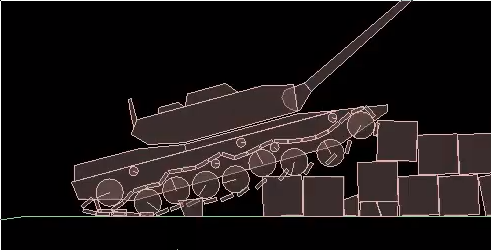
\includegraphics[width=10cm]{box2dDebug}
	\caption{Izrisovanje fizikalnih teles za potrebe razhroščevanja. Vir \cite{box2dTank}}
	\label{slika:box2dDebug}
\end{figure}

Unity podpira dva fizikalna pogona. Za 2D simulacijo ima integriran in razširjen Box2D, za 3D simulacija pa modificiran PhysX. Uporaba fizikalnega pogona v Unity je zelo preprosta, saj našim objektov v igri dodamo komponento \textit{togo telo}. Unity v večini primerov poskrbi, da se konstrukcija sklada z izrisanim objektom in ponuja vizualno urejanje konstrukcije, če je to potrebno. Na sliki \ref{slika:unityRigidbody} vidimo primer dela z fizikalnim pogonom. Žoga vidna na levi prikazuje svojo konstrukcijo v zeleni barvi. Na desni pa vidimo komponente igralnega objekta, za fizikalno simulacijo sta pomembna \textit{Konstrukcija krogle} () in \textit{RigidBody} (togo telo). Komponentam lahko nastavimo lastnosti konstrukcije in telesa, ki smo jih omenili zgoraj. V kodi lahko sledimo trkom v metodah \textit{OnTriggerEnter()} in \textit{OnCollissionEnter()}, ki nam podajo vse potrebne informacije o trkih, nakar lahko mi dodamo svoje kodo odvisno na dogajanje.

\begin{figure}[h]
	\centering
	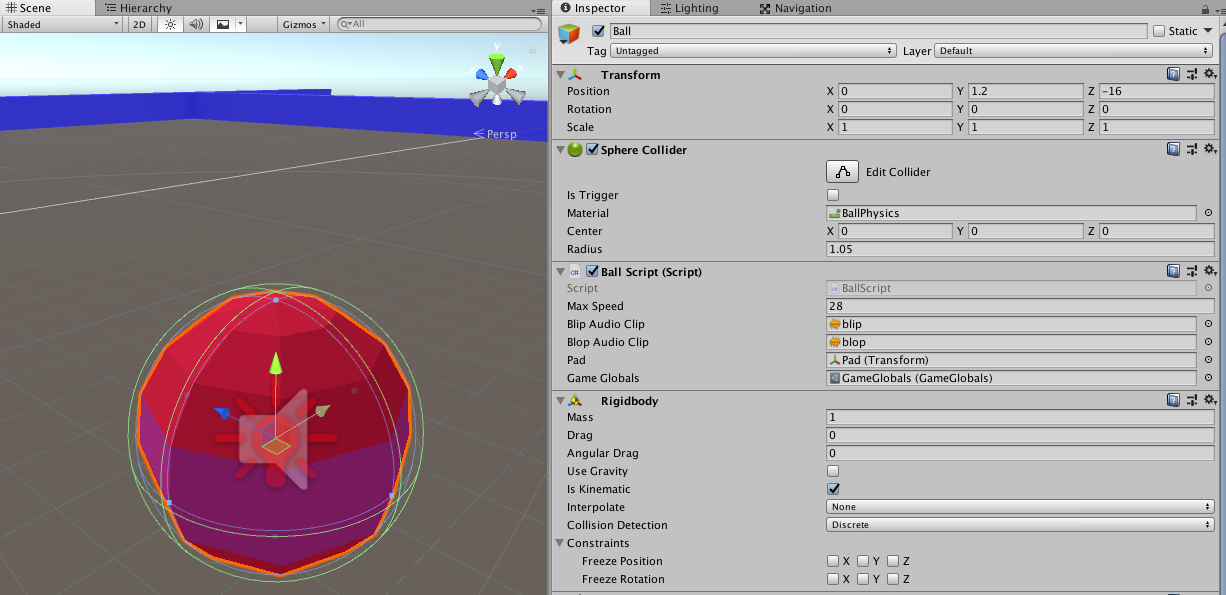
\includegraphics[width=15cm]{unityRigidbody}
	\caption{Urejanje konstrukcije in togega telesa na igralnem objektu}
	\label{slika:unityRigidbody}
\end{figure}

\subsection{Umetna inteligenca v igrah}
Na kratko samo, potem pa pathfinding.

\subsection{Unity ProBuilder}
Malo o tool

\chapter{Sklep}\thispagestyle{fancy}

\cleardoublepage
\bibliographystyle{plain}
\bibliography{thesis}
\addcontentsline{toc}{chapter}{Literatura}

\end{document}